\documentclass[12pt,a4paper]{report}
\usepackage[utf8]{inputenc}
\usepackage[T1]{fontenc}
\usepackage{lmodern}
\usepackage{graphicx}
\usepackage{geometry}
\usepackage{setspace}
\usepackage{titlesec}
\usepackage{array}
\usepackage{float}
\usepackage{tabularx}
\usepackage{longtable}
\usepackage{amsmath}
\usepackage{url}
\usepackage{hyperref}
\geometry{a4paper, margin=1in}
\graphicspath{{images/}}
\emergencystretch=3em
\newcolumntype{L}[1]{>{\raggedright\arraybackslash}p{#1}}

\begin{document}

% 1. Front page
\begin{titlepage}
    \begin{center}
        
\includegraphics[width=0.7\textwidth]{MITS_LOGO.pdf} \\
        % \vspace*{1cm}

        \Huge
        \textbf{VibeStack} \\[0.3cm]
        \LARGE\textbf{An Architecture-Aware AI Software Engineering Harness} \\
        \vspace{1cm}

        \large
        Project Phase I Report submitted in partial fulfillment for the degree \\
        of \\
        \textbf{B.Tech in CSE(Artificial Intelligence) } \\
        \vspace{0.5cm}

        Submitted by \\
        \textbf{Reuben Sabu V (Reg No: MUT23CA060)} \\
        \textbf{Sidharth Ravi (Reg No: MUT23CA063)} \\
        \textbf{Jino Jenz (Reg No: MUT23CA035)} \\
        \textbf{Nikhil Jimmy (Reg No: MUT23CA055)} \\

        % \vfill
        \vspace{1cm}
        \Large
        \textbf{Muthoot Institute of Technology and Science Kochi (Autonomous)} \\

        \vspace{0.5cm}
        \textbf{Department of Artificial Intelligence and Data Science} \\
        (Affiliated to APJ Abdul Kalam Technological University) \\
        \vspace{0.5cm}
        \textbf{OCTOBER 2026}
    \end{center}
\end{titlepage}

\pagenumbering{roman}

% 2. Certificate
% 2. Certificate
\newpage
\addcontentsline{toc}{chapter}{Certificate}
\begin{center}
    
\includegraphics[width=0.7\textwidth]{MITS_LOGO.pdf} \\
    \vspace{0.5cm}
    \textbf{DEPARTMENT OF ARTIFICIAL INTELLIGENCE AND DATA SCIENCE} \\
    \vspace{1cm}
    \Large\textbf{CERTIFICATE}
\end{center}
\vspace{1cm}

This is to certify that the Project Phase I report entitled \textbf{"VibeStack: An Architecture-Aware AI Software Engineering Harness"}, submitted by Reuben Sabu V (MUT23CA060), Sidharth Ravi (MUT23CA063), Jino Jenz (MUT23CA035), Nikhil Jimmy (MUT23CA055) of Semester VII is a bonafide account of the work done by them under our supervision during the academic year 2026-27.

\vspace{3cm}
% \noindent
\begin{center}
\begin{tabular}{p{0.30\textwidth} p{0.30\textwidth} p{0.50\textwidth}}
\textbf{Guide} &
\textbf{Coordinator(s)} &
\textbf{Head of the Department} \\[4pt]

Nimmi M K &
Dr. Parvathy Jyothi / Ms. Angel Varghese  &
Dr. Cerene Mariam Abraham \\

Assistant Professor &
Asst. Professor &
Associate Professor \\

Dept. of AI\&DS &
Dept. of AI\&DS &
Dept. of AI\&DS
\end{tabular}
\end{center}

\newpage
% 3. Declaration
\newpage
\addcontentsline{toc}{chapter}{Declaration}
\begin{center}
    \Large\textbf{DECLARATION}
\end{center}
\vspace{1cm}

% \chapter*{DECLARATION}
% \addcontentsline{toc}{chapter}{Declaration}
We hereby declare that this submission is our own work and that, to the best of our knowledge and belief, it contains no material previously written by another person nor material which has been accepted for the award of any other degree or diploma of the university or other institute of higher learning, except where due acknowledgement has been made in the text.
\par\vspace{0.5cm}
\noindent
The overall similarity index as per the Turnitin plagiarism check is \textbf{XX\%}.

\vspace{1.5cm}
\noindent Reuben Sabu V (Reg No: MUT23CA060) \\
Sidharth Ravi (Reg No: MUT23CA063) \\
Jino Jenz (Reg No: MUT23CA035) \\
Nikhil Jimmy (Reg No: MUT23CA055) \\

\vspace{1cm}
\noindent Place: Kochi \\
Date:

\newpage
% 4. Acknowledgement

% 4. Acknowledgement
\newpage
\addcontentsline{toc}{chapter}{Acknowledgement}
\begin{center}
    \Large\textbf{ACKNOWLEDGEMENTS}
\end{center}
\vspace{1cm}
\noindent
This project report is the result of our hard work wherein we have been helped and supported by several persons and institutions directly and indirectly. Now it is the time to acknowledge their valuable contributions.
\par\vspace{0.5cm}
\noindent
We would like to extend our sincere gratitude to the Management of Muthoot Institute of Technology and Science for providing us with the necessary facilities, resources, and a conducive environment to carry out our project successfully.
\par\vspace{0.5cm}
\noindent
We are deeply thankful to Dr. Neelakantan P. C., Principal, Muthoot Institute of Technology and Science, for his constant support, guidance, and encouragement throughout our academic journey. Our sincere gratitude to Dr. Cerene Mariam Abraham, Head of the Department during our course period, for her guidance and support. Her encouragement and leadership have greatly helped us in successfully completing our project.
\par\vspace{0.5cm}
\noindent
We would like to express our heartfelt gratitude to our project guide, Nimmi M K, Assistant Professor, Department of Artificial Intelligence and Data Science, for the continuous encouragement, invaluable guidance, motivation, and enthusiasm shown throughout our project. We would also like to thank the project coordinators Dr. Parvathy Jyothi and  Ms. Angel Varghese, for critically assessing our work and providing valuable suggestions.
\par\vspace{0.5cm}
\noindent
Besides this, several people have knowingly and unknowingly helped us in the successful completion of this project. We express our sincere gratitude to all of them.



\newpage
% 6. Abstract
\chapter*{Abstract}
\addcontentsline{toc}{chapter}{Abstract}

AI coding assistants can now write hundreds of lines of code in seconds, but the code they hand back is rarely checked. For a multi-file backend this is a real problem: a wrong import, a missing foreign key or a forgotten permission check only shows up when someone tries to run the application, and finding the cause often takes longer than writing the code by hand. Most of the popular ``app builder'' tools are also built around JavaScript stacks, which leaves Python backend developers with little support.

VibeStack is our answer to this. It is a harness that turns a plain-English description of an application into a working, tested, full-stack web application with a Python backend (FastAPI, Flask or Django) and a React frontend. Instead of one large prompt, the work is split across eight agents wired together as a LangGraph state machine: an Architect, a Planner, a Code Generator, a Validator, an Error Classifier, a Reflector, a Packager and a Circuit Breaker. Three design decisions keep the output reliable. First, everything that can be written once and verified (models, schemas, routers, authentication and the frontend) comes from tested templates, and the language model writes only the business logic. Second, every generated application is executed in an isolated sandbox and must pass four gates in order: static analysis, import, boot and tests. The tests include contract tests, edge-case tests derived from the design without any AI, and business-rule tests that are written before the code exists. Third, when a gate fails, a self-healing loop classifies the error, locates the faulty file and repairs it with a tool-using agent. The loop does not stop after a fixed number of tries. It continues while each repair makes measurable progress, escalates from a cheap model to a strong model to the verified template when it stalls, and rolls back repairs that make things worse. Every agent action is recorded in a change ledger with the exact diff.

At the time of writing, the harness, the web platform and an automated test suite of about 120 tests are complete and merged. In the interim evaluation, a real end-to-end run produced a working blog backend with JWT authentication in about 51 seconds for less than one US cent, and all ten benchmark projects in the harness evaluation were repaired successfully. A full benchmark of fifteen prompts on real models, with ablation studies, is the main task for the next phase.

\vspace{0.5cm}
\noindent\textbf{Keywords:} Large language models, multi-agent systems, code generation, self-healing software, automated testing, LangGraph, FastAPI.


\newpage
% 7. Contents
\tableofcontents

\newpage
% 8. List of Figures
\listoffigures
\addcontentsline{toc}{chapter}{List of Figures}

\newpage
% 9. List of Tables
\listoftables
\addcontentsline{toc}{chapter}{List of Tables}

\newpage
\pagenumbering{arabic}
\doublespacing

% 10. Chapter 1- Introduction
\chapter{Introduction}
\section{Background}

Large language models (LLMs) trained on source code have changed how software is written. Tools such as GitHub Copilot \cite{copilot} complete functions as the developer types, and newer ``app builders'' promise to produce an entire application from a short description. Research systems have pushed the same idea further. Codex \cite{chen2021codex} showed that a model can solve a large share of short programming problems, and multi-agent systems such as MetaGPT \cite{hong2024metagpt} and ChatDev \cite{qian2024chatdev} split software development into roles played by different agents.

In our own use of these tools during earlier coursework and hackathons, we kept running into the same pattern. The first draft looks complete, but it has not been run. When it is run, something small breaks: an import points to a file that was never created, a database relation is defined on one side only, or an endpoint returns the wrong status code. Each of these is easy to fix once found, but finding them in a project of twenty or thirty files written by someone else (in this case, a model) is slow. The time saved by generating the code is often lost again while debugging it.

A second observation shaped the project. The best-known app builders target JavaScript stacks such as React with Node.js. Python is the most common language for data and AI work, and FastAPI, Flask and Django are widely used for backends, yet there was no comparable tool that understood these frameworks and their conventions natively and that a developer could run on their own machine or server.

VibeStack started from these two observations. Rather than trying to make the model write better code in one attempt, we built a harness around it that does what a careful developer would do: plan the design, write the code, run it, read the error, fix the right file, and run it again. The model is only one part of the system. The rest is ordinary, deterministic software that checks the model's work.

\section{Problem Statement}

To address the lack of AI-powered, deployment-ready application builders tailored for Python backend developers by overcoming the JavaScript-centric bias of existing tools, and to build a reliable, locally installable or deployable backend generation system that natively understands Python frameworks and conventions, giving developers full control over their infrastructure and code without dependency on third-party cloud services.

Stated as an engineering problem: AI code generators produce unverified and often inconsistent multi-file backends. We need a harness that designs, executes, tests and repairs generated code \emph{before} it is delivered, and that explains every change it makes.

\section{Objectives}

The objectives of the project are:

\begin{enumerate}
    \item To design a multi-agent pipeline of eight specialised agents that converts a natural-language application description into a deployable full-stack web application, with a React frontend and a FastAPI, Flask or Django backend.
    \item To verify generated applications automatically through static analysis, sandboxed execution, design-derived contract and edge-case tests, business-rule tests written before the code, and a frontend--backend contract check.
    \item To repair defects autonomously with a progress-driven self-healing loop that needs no fixed iteration limit, using a tool-augmented repair agent that can inspect code and run tests.
    \item To support iterative development, in which follow-up requests produce new, versioned applications that reuse unchanged components.
    \item To evaluate the system on a benchmark of 15 applications across three frameworks, with ablations that measure the contribution of dynamic healing, tool use and design-derived tests to success rate, escaped defects, cost and time.
    \item To make the system extensible and interoperable through a plugin interface and the Model Context Protocol (MCP), as both server and client.
\end{enumerate}

\section{Scope}

The project focuses on CRUD-style web applications with business rules: systems built around entities, relations, permissions and actions such as booking, checkout or approval. Generated applications use SQLAlchemy 2.0 (FastAPI and Flask) or the Django ORM, JWT-based authentication \cite{rfc7519}, and a React frontend. Each one comes with tests, database migrations, a Dockerfile and a CI configuration. The platform itself is a web application with live progress, a live preview of the generated app and one-click deployment. Mobile apps, desktop software and arbitrary algorithmic programs are outside the scope.

\section{Relevance to Sustainable Development Goals}

Following the suggestion of the zeroth review committee, the project is mapped to a single goal: \textbf{SDG 9, Industry, Innovation and Infrastructure} \cite{un_sdg9}, specifically \textbf{Target 9.5}, which calls for enhancing research and upgrading the technological capabilities of industry. VibeStack makes reliable, verified software engineering accessible to students, small teams and start-ups that cannot afford a large engineering team.

\section{Organisation of the Report}

Chapter~2 reviews existing tools and research on LLM-based code generation and self-repair and identifies the gap this project addresses. Chapter~3 presents the system architecture, the modules and the algorithms used in each. Chapter~4 describes how the system has been implemented. Chapter~5 reports the preliminary results. Chapter~6 gives the project schedule, and Chapter~7 concludes the report and outlines the work planned for Phase II.

% 11. Chapter 2- Literature Review
\chapter{Literature Review}
\section{Introduction}

Our literature survey covered fifteen sources: research papers on LLM agents, self-correction and automated software engineering, plus the documentation of the frameworks we build on. This chapter summarises the most relevant ones. For each paper, we note the core idea, how it was evaluated and the limitation that matters for our problem. We close the chapter with the gaps we found and a comparison against our proposed system.

\section{Related Work}
\subsection{Existing System}

Existing tools fall roughly into three groups.

\textbf{Code completion assistants} such as GitHub Copilot \cite{copilot} work inside the editor and suggest the next few lines or a whole function. They are very good at local code but have no view of the whole project and never run what they write. Checking the result is left entirely to the developer.

\textbf{Prompt-to-project generators} such as gpt-engineer \cite{gptengineer} take a description and write a full set of files. Some ask clarifying questions first. In most of them, however, the output is generated in one pass and handed over without being executed, so the developer receives a project that may not even start.

\textbf{Hosted app builders} generate a running application inside the vendor's cloud and are mostly built around JavaScript stacks. They do run the code, but the developer depends on the vendor's infrastructure, has limited control over the backend, and gets little explanation of why the code looks the way it does.

None of these groups combines a Python-first backend, execution-based verification, automatic repair and a record of what was changed and why.

\subsection{Reflexion: Language Agents with Verbal Reinforcement Learning (N. Shinn et al., NeurIPS, 2023)}

Reflexion \cite{shinn2023reflexion} lets an agent learn from failure without updating model weights. After each attempt, the agent receives feedback (for code, the result of unit tests), writes a short verbal reflection on what went wrong, and stores it in memory for the next attempt. On the HumanEval coding benchmark this raised the pass rate well above a single attempt.

\textbf{Limitations:} Reflexion works on single functions with given tests. The number of trials is fixed in advance, and the agent edits the whole solution rather than locating the faulty part. It does not address multi-file projects in which the error and its cause are in different files.

\subsection{Teaching Large Language Models to Self-Debug (X. Chen, M. Lin, N. Sch{\"a}rli and D. Zhou, ICLR, 2024)}

Self-Debug \cite{chen2024selfdebug} teaches a model to debug its own code through few-shot prompting. The model executes the code, explains it line by line (``rubber duck debugging'') and uses the execution result to produce a corrected version. The paper reports consistent gains on text-to-SQL, code translation and Python programming tasks.

\textbf{Limitations:} The technique is evaluated on self-contained snippets. There is no notion of a project layout, of which file to fix, or of when to stop when repairs no longer help.

\subsection{CRITIC: Large Language Models Can Self-Correct with Tool-Interactive Critiquing (Z. Gou et al., ICLR, 2024)}

CRITIC \cite{gou2024critic} argues that models are poor at judging their own output from introspection alone, but improve when they can verify it with external tools such as a search engine or a code interpreter. The model generates an answer, uses tools to critique it, and revises it.

\textbf{Limitations:} CRITIC shows why tools matter for correction, but it is a general framework evaluated on question answering, mathematics and toxicity. It does not deal with building and testing software projects.

\subsection{ReAct: Synergizing Reasoning and Acting in Language Models (S. Yao et al., ICLR, 2023)}

ReAct \cite{yao2023react} interleaves reasoning steps with actions such as calling a tool and observing the result. This pattern is now the basis of most tool-using agents, including our repair agent, which reads files, searches code and runs tests before proposing a fix.

\textbf{Limitations:} ReAct is a prompting pattern, not a software engineering system. It gives no guidance on verification, test oracles or limiting the cost of long loops.

\subsection{SWE-bench: Can Language Models Resolve Real-World GitHub Issues? (C. E. Jimenez et al., ICLR, 2024)}

SWE-bench \cite{jimenez2024swebench} is a benchmark of real GitHub issues from popular Python repositories. A model must produce a patch that makes the repository's hidden tests pass. It showed that resolving real issues in large codebases is much harder than solving isolated problems.

\textbf{Limitations:} SWE-bench evaluates the repair of existing human-written code. It does not cover generating a new project, and it assumes a trustworthy test suite already exists. In generation from scratch, the tests themselves must also be produced and checked.

\subsection{SWE-agent: Agent-Computer Interfaces Enable Automated Software Engineering (J. Yang et al., NeurIPS, 2024)}

SWE-agent \cite{yang2024sweagent} shows that the interface given to an agent matters as much as the model. With a small set of well-designed commands for viewing, searching and editing files, plus feedback from running code, a model resolves many more SWE-bench issues than with a raw shell.

\textbf{Limitations:} SWE-agent edits existing repositories and stops based on a cost or step budget. Our Reflector borrows its idea of a small, purpose-built toolset, but applies it to code that the system generated itself.

\subsection{AgentCoder: Multi-Agent Code Generation with Iterative Testing and Optimisation (D. Huang et al., arXiv:2312.13010, 2023)}

AgentCoder \cite{huang2023agentcoder} uses three agents: a programmer, a test designer and a test executor. The test designer writes tests independently of the programmer, so the tests are not biased by the code, and the executor feeds failures back to the programmer.

\textbf{Limitations:} The tests are still written by a language model, so they can be wrong, and nothing checks them. Evaluation is on function-level benchmarks rather than multi-file applications, and the loop runs for a fixed number of iterations.

\subsection{Evaluating Large Language Models Trained on Code (M. Chen et al., arXiv:2107.03374, 2021)}

This paper introduced Codex and the HumanEval benchmark, and established functional correctness, measured by running unit tests (pass@k), as the standard way to evaluate generated code instead of text similarity.

\textbf{Limitations:} HumanEval problems are single functions. The paper itself notes that models struggle with long specifications and multi-step logic, which is exactly where application generation lives.

\subsection{MetaGPT: Meta Programming for a Multi-Agent Collaborative Framework (S. Hong et al., ICLR, 2024)}

MetaGPT \cite{hong2024metagpt} encodes standard operating procedures from human software companies into a team of agents (product manager, architect, engineer, QA) that exchange structured documents rather than free chat. Structured hand-offs reduced the inconsistencies seen in chat-based multi-agent systems.

\textbf{Limitations:} The generated projects are not always executable, and the QA step relies on the model rather than on independent checks. There is no explicit repair strategy with a stopping rule.

\subsection{ChatDev: Communicative Agents for Software Development (C. Qian et al., ACL, 2024)}

ChatDev \cite{qian2024chatdev} models a virtual software company in which agents in different roles talk through design, coding and testing phases. It produces small applications cheaply and quickly.

\textbf{Limitations:} The output is mostly small single-user programs. Verification is conversational, and the cost of long dialogues grows quickly. There is no target framework or deployment story for backend services.

\section{Gaps in Literature}

Reading these works together, we found five gaps that matter for building reliable backends:

\begin{enumerate}
    \item \textbf{Scale of the target.} Most self-repair research works on single functions. Multi-file applications, where the error message and its cause are in different files, are rarely addressed.
    \item \textbf{When to stop.} Almost every repair loop uses a fixed number of attempts or a step budget. A fixed limit either gives up on a repair that was making progress or keeps paying for one that is stuck.
    \item \textbf{Trustworthy tests.} When the model writes both the code and the tests, a wrong test can drive the repair in the wrong direction. Few systems have an independent oracle that does not depend on the model.
    \item \textbf{How much the model writes.} Existing generators ask the model to write everything, including boilerplate that could be written once and verified.
    \item \textbf{Explainability and ownership.} Generated code is usually handed over without a record of why it was written or changed, and hosted tools keep the code and infrastructure in the vendor's cloud.
\end{enumerate}

Table~\ref{tab:comparison} compares representative systems with VibeStack against these points.

\begin{table}[!ht]
    \centering
    \renewcommand{\arraystretch}{1.3}
    \footnotesize
    \caption{Comparison of existing systems with the proposed system}
    \label{tab:comparison}
    \begin{tabular}{|L{2.4cm}|L{1.6cm}|L{1.6cm}|L{1.6cm}|L{1.9cm}|L{2.0cm}|L{1.8cm}|}
    \hline
    \textbf{System} & \textbf{Multi-file app} & \textbf{Runs the code} & \textbf{Self-repair} & \textbf{Stopping rule} & \textbf{Independent test oracle} & \textbf{Change ledger} \\\hline
    Copilot \cite{copilot} & No & No & No & -- & No & No \\\hline
    Reflexion \cite{shinn2023reflexion} & No & Yes & Yes & Fixed trials & No & No \\\hline
    Self-Debug \cite{chen2024selfdebug} & No & Yes & Yes & Fixed turns & No & No \\\hline
    AgentCoder \cite{huang2023agentcoder} & No & Yes & Yes & Fixed iterations & No (LLM tests) & No \\\hline
    MetaGPT \cite{hong2024metagpt} & Yes & Partly & Limited & -- & No & Documents only \\\hline
    SWE-agent \cite{yang2024sweagent} & Existing repo & Yes & Yes & Cost budget & Given tests & Trajectory log \\\hline
    \textbf{VibeStack} & \textbf{Yes, full-stack} & \textbf{Yes, sandboxed} & \textbf{Yes, tool-using} & \textbf{Progress-driven} & \textbf{Yes, design-derived} & \textbf{Yes, with diffs} \\\hline
    \end{tabular}
\end{table}

VibeStack addresses these gaps by (i) generating complete multi-file applications but letting the model write only the business logic, (ii) replacing the fixed attempt limit with a progress-based stopping rule, (iii) deriving edge-case tests from the design without any AI, so they act as an independent oracle, (iv) calibrating the model-written tests against verified code before use, and (v) recording every change in a ledger, with all code staying under the developer's control.


% Chapter 3- System Design

\chapter{System Design}
\section{System Architecture}

VibeStack is organised into four layers, shown in Fig.~\ref{fig:architecture}.

\begin{figure}[!ht]
	\centering
		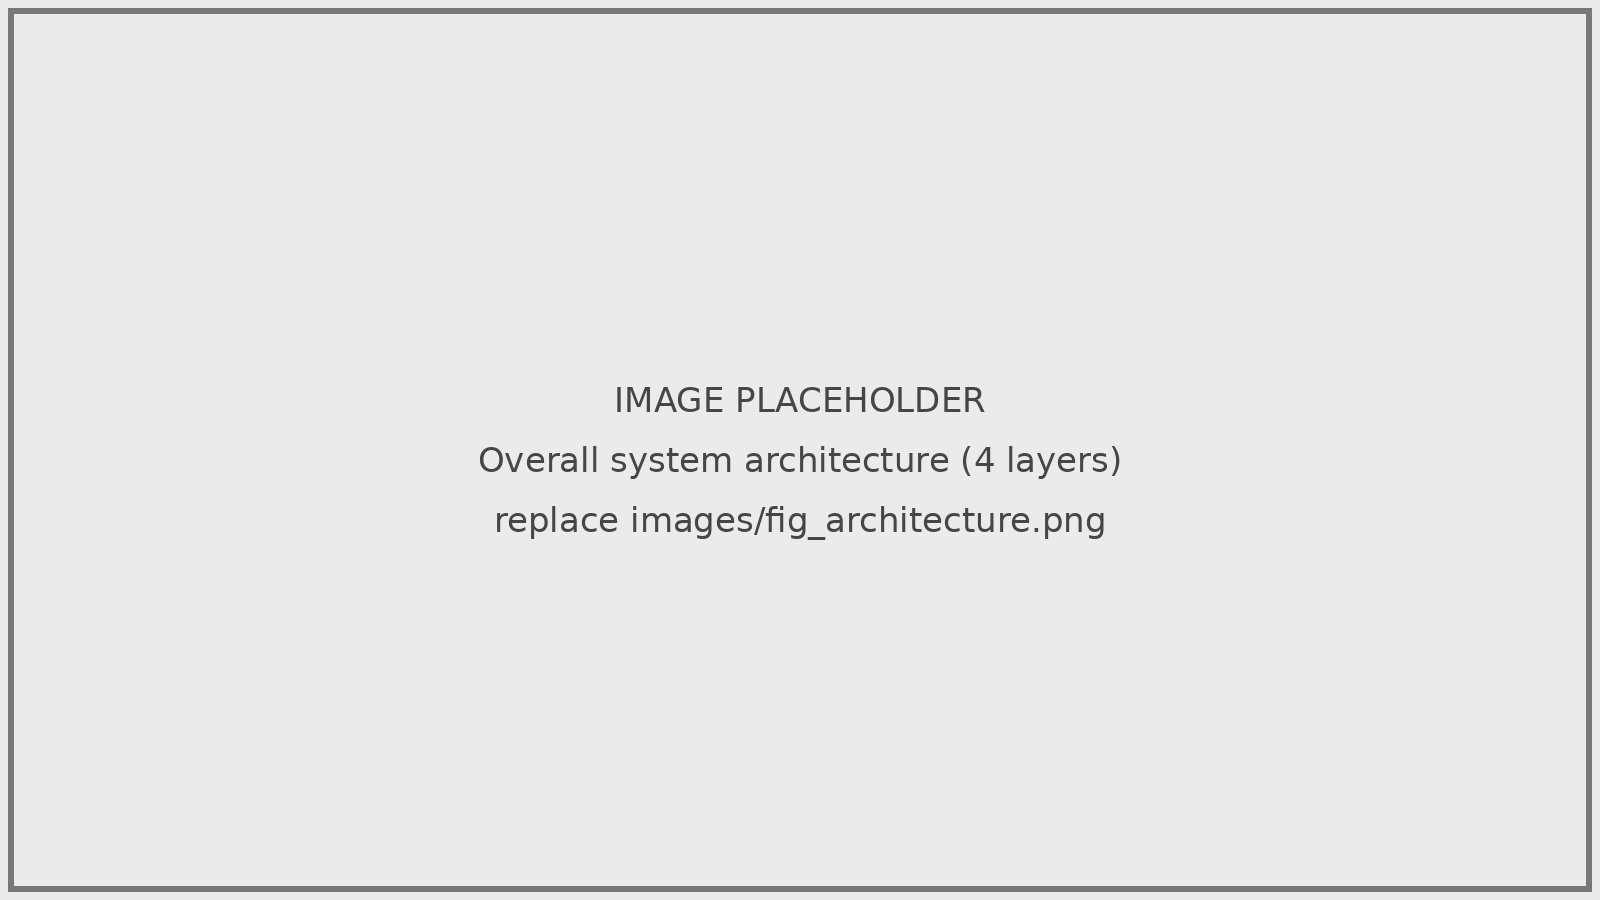
\includegraphics[width=0.95\textwidth]{fig_architecture.png}
	\caption{Overall system architecture of VibeStack}
	\label{fig:architecture}
\end{figure}

\begin{enumerate}
    \item \textbf{Presentation layer.} A Next.js web interface \cite{nextjs} where the user describes the application, reviews the design, watches the agents work, inspects the code, the tests and the ledger, and uses the generated app in a live preview. The interface is exported as static files and served by the backend, so a single container runs the whole platform.
    \item \textbf{Application layer.} A FastAPI service \cite{fastapi} that manages accounts, projects and versions. It starts builds through the run manager, streams agent progress to the browser with Server-Sent Events (SSE), and proxies the live preview of each generated app at a private \texttt{/preview/<key>/} address. It also exposes an MCP server so that external AI tools can drive VibeStack \cite{mcp}.
    \item \textbf{Orchestration layer.} The eight agents, connected as a LangGraph \cite{langgraph} state machine. LangGraph was chosen because the self-healing cycle is a loop with conditional exits, and because it saves a checkpoint after every step, so an interrupted build can resume where it stopped.
    \item \textbf{Infrastructure and data layer.} The LLM provider API (Gemini by default, or Groq, OpenRouter \cite{openrouter} or any OpenAI-compatible endpoint), the isolated sandbox that executes generated code, the checkpoint and platform database (SQLite locally, PostgreSQL in production) and the storage for generated artifacts (local disk or any S3-compatible bucket).
\end{enumerate}

The flow through the orchestration layer is shown in Fig.~\ref{fig:flowchart}. A build moves from the Architect to the Planner, the Code Generator and the Validator. If every gate passes, the Packager delivers the app. If a gate fails and healing is still making progress, the Error Classifier and the Reflector repair the code and send it back to the Validator. If healing stops making progress, the Circuit Breaker ends the run with a diagnostic report.

\begin{figure}[!ht]
	\centering
		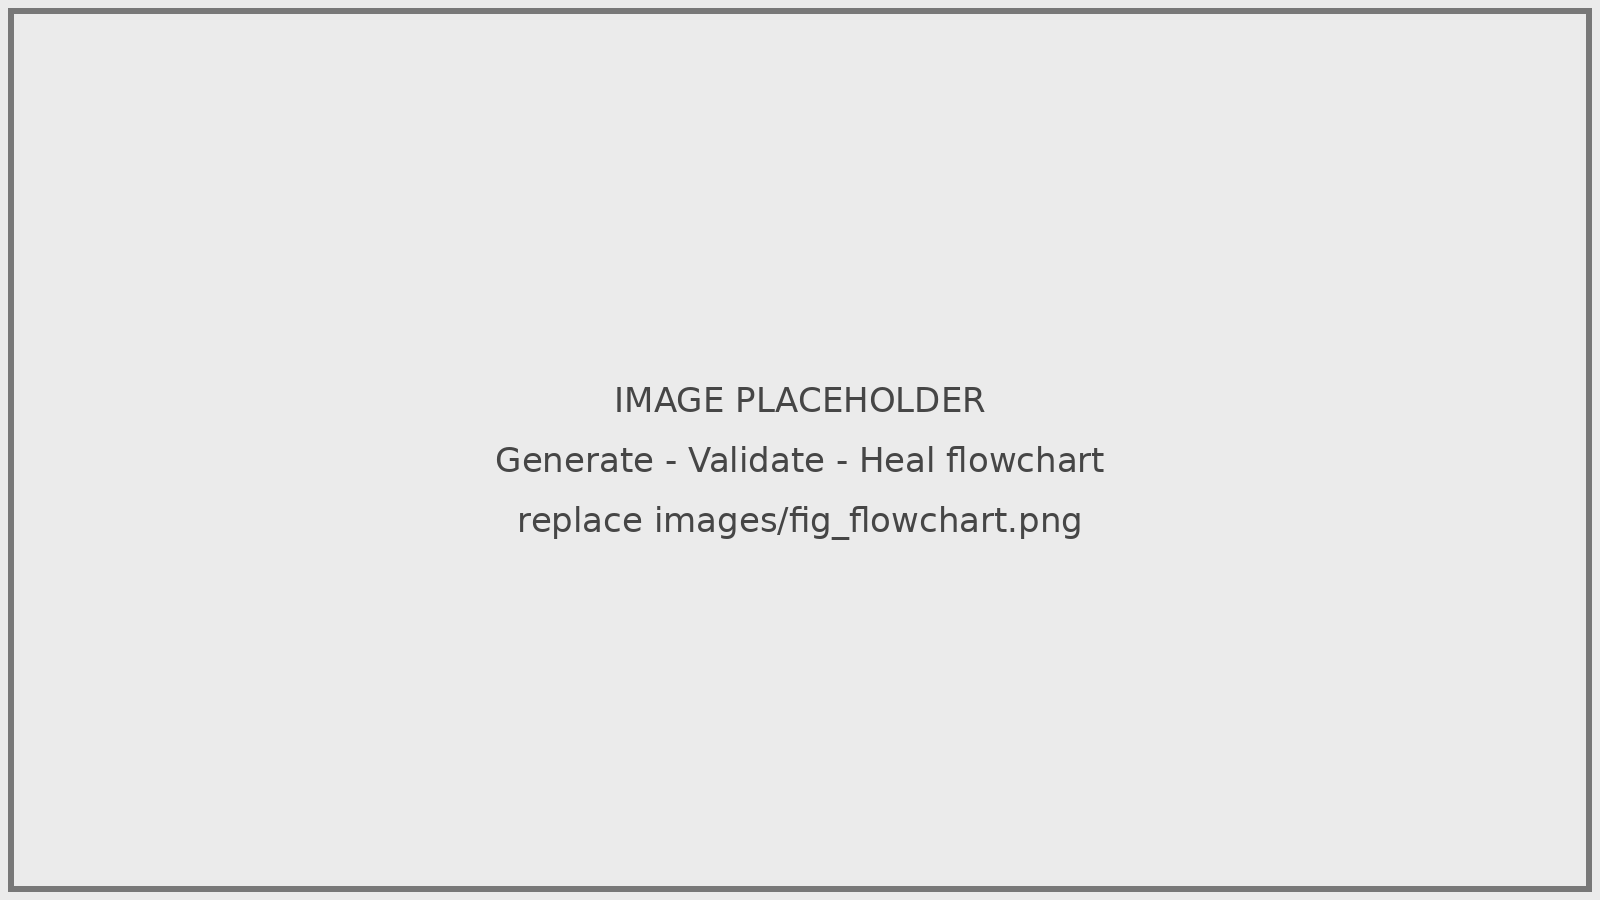
\includegraphics[width=0.85\textwidth]{fig_flowchart.png}
	\caption{Flowchart of the Generate $\rightarrow$ Validate $\rightarrow$ Heal algorithm}
	\label{fig:flowchart}
\end{figure}

\section{Modules}

Fig.~\ref{fig:modules} shows the main modules. Each agent is a single Python function in \texttt{backend/agent/nodes.py} that reads the shared state and returns the fields it changes. This section describes what each module does and the algorithm behind it. We give the file and function names so that every step can be checked against the source code.

\begin{figure}[!ht]
	\centering
		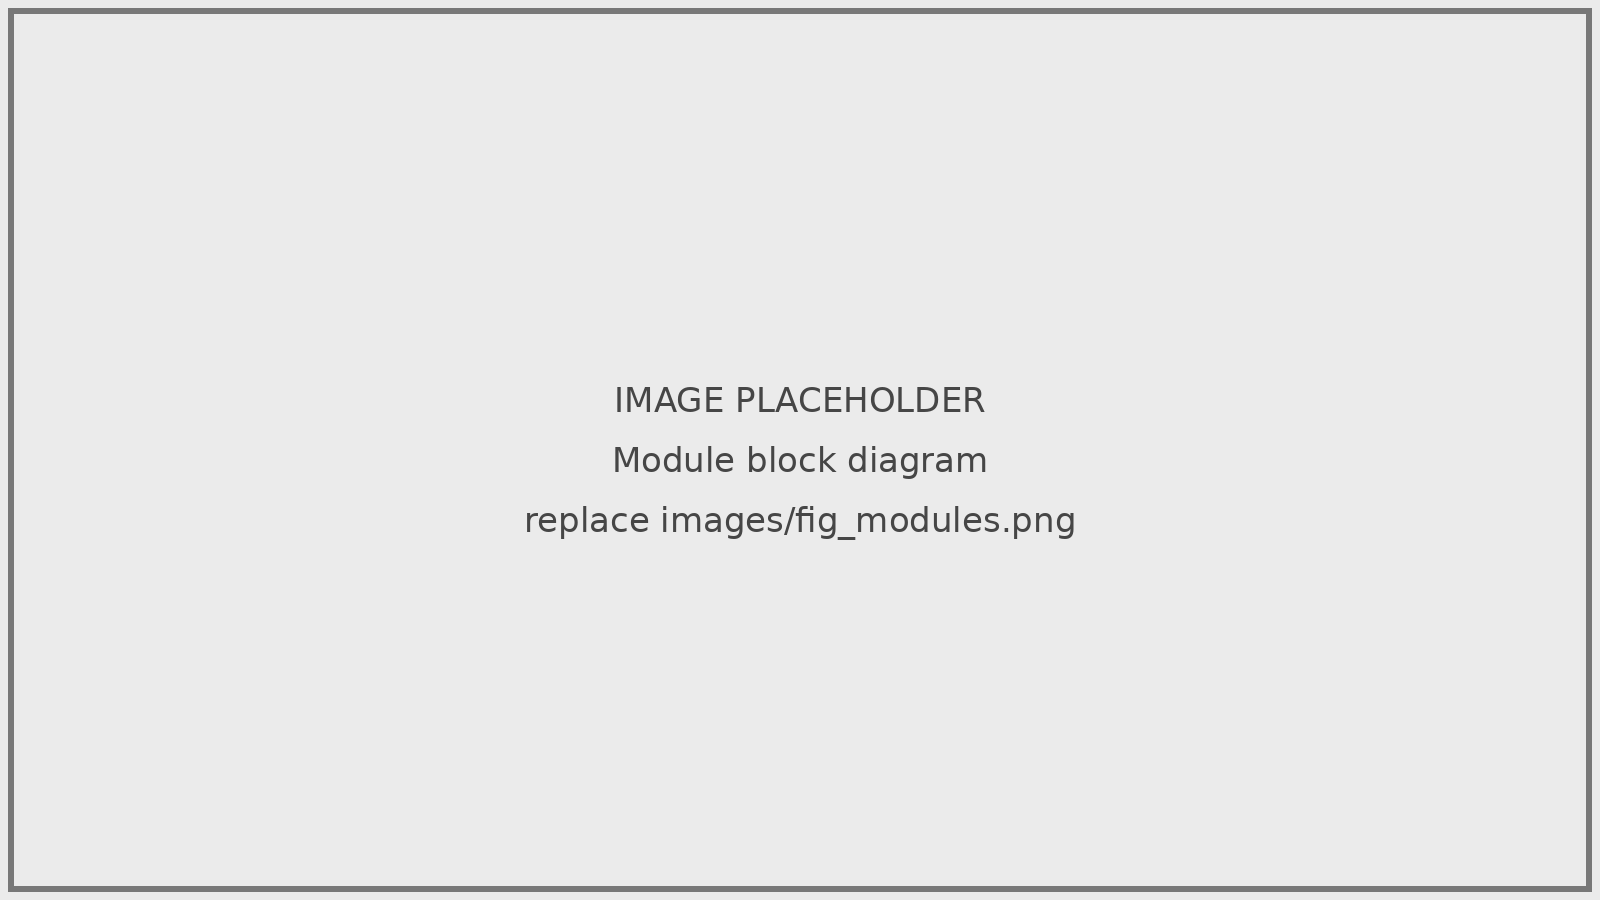
\includegraphics[width=0.75\textwidth]{fig_modules.png}
	\caption{Module block diagram}
	\label{fig:modules}
\end{figure}

\subsection{Architect (Requirement Analysis and Design)}

The Architect (\texttt{parse\_spec}) converts the user's description into a structured design called a \texttt{ProjectSpec} (\texttt{agent/state.py}). The spec is a Pydantic \cite{pydantic} model, so any output that does not match the schema is rejected immediately rather than discovered later as broken code. A spec contains:

\begin{itemize}
    \item \textbf{Entities} with typed fields (\texttt{str}, \texttt{text}, \texttt{int}, \texttt{float}, \texttt{decimal}, \texttt{bool}, \texttt{date}, \texttt{datetime}, \texttt{json}), uniqueness, indexes and foreign keys with delete rules (\texttt{cascade}, \texttt{restrict}, \texttt{set\_null}).
    \item \textbf{State machines} on enum fields, for example \texttt{draft} $\rightarrow$ \texttt{running} $\rightarrow$ \texttt{done}. A forbidden transition must return HTTP 409.
    \item \textbf{Access rules} per entity (\texttt{any\_user}, \texttt{owner} or \texttt{admin}) and named \textbf{roles}.
    \item \textbf{Custom actions} with business rules, such as \texttt{POST /orders/\{id\}/checkout}.
    \item A numbered list of \textbf{requirements}, each linked to the entity or action that covers it, and the \textbf{plugins} the build needs, with a reason for each.
\end{itemize}

\noindent\textbf{Algorithm 1: Architect}
\begin{enumerate}
    \item Send the prompt, any project rules and, for a follow-up, the previous design to the strong model with the design prompt.
    \item Parse the JSON reply into a \texttt{ProjectSpec}. If parsing fails, send the validation error back once for a repair round-trip.
    \item Normalise the spec, for example by turning on authentication when an entity needs owners or admins.
    \item If the spec has custom actions, ask the model to write \textbf{business-rule tests} now, before any code exists (\texttt{testwriter.write\_rule\_tests}).
    \item For a follow-up request, compute what changed between the old and new design (\texttt{design\_changes}) so that only the changed parts are regenerated.
\end{enumerate}

\subsection{Planner and Design Review}

The Planner (\texttt{plan}) orders the files to be generated by dependency: database and configuration first, then models, schemas, services and routers, then the application entry point and the tests. When design review is turned on, the build pauses here. The user sees an entity diagram, a role-by-table permission matrix, the feature toggles and the actions, and can approve the design, edit it, or ask for a change in words. A change in words sends the build back to the Architect. No code is generated until the design is approved.

\subsection{Code Generator}

The most important design decision in VibeStack is how little code the model writes. Models, schemas, routers, authentication, error handling and the React frontend follow patterns that do not change from one app to the next, so they are produced from verified Jinja2 templates (\texttt{agent/templates/}). These templates have been tested against the contract tests for all three frameworks. The model writes only the \textbf{business logic}: one service file per entity that has custom actions (\texttt{app/services/<entity>.py}), plus a small \texttt{ui.json} that controls the look of the app.

\noindent\textbf{Algorithm 2: Code Generator}
\begin{enumerate}
    \item Render every template file for the chosen framework (\texttt{codegen.py}, \texttt{stacks.py}).
    \item Derive the \textbf{edge-case tests} from the design, without any model: an unknown foreign key must return 409, a forbidden state change 409, another user's row 404, an out-of-range value 422, and so on.
    \item For each entity with actions, ask the model, in parallel, to write the service file, giving it only that entity's context (\texttt{\_generate\_service}).
    \item Check each generated file with Python's \texttt{ast} parser. A syntax error gets one cheap repair call before validation (\texttt{\_fix\_syntax}).
    \item Store the template output separately, so the healing loop can later restore any file to its verified version.
\end{enumerate}

Because only the business-logic files are model-written, the helper \texttt{healing.editable()} lets the repair agent change only those files and \texttt{ui.json}. Everything else is protected.

\subsection{Validator (Sandbox Execution)}

The Validator (\texttt{validate}, \texttt{agent/sandbox.py}) writes the project to a temporary directory and runs four gates, cheapest first. The first gate that fails stops validation, and its log is passed on.

\begin{enumerate}
    \item \textbf{Static gate.} AST checks from \texttt{agent/bughunt.py} for \texttt{eval}/\texttt{exec}, shell commands, hard-coded secrets, SQL built from strings, hard-coded debug mode, bare \texttt{except} and stray \texttt{print}. The frontend contract check (\texttt{frontend.check\_frontend}) runs here too: everything the React app uses must exist in the backend.
    \item \textbf{Import gate.} Import the application module. This catches syntax errors, missing modules and broken ORM mappings.
    \item \textbf{Boot gate.} Start the server on a free port and wait for \texttt{/health} to answer.
    \item \textbf{Test gate.} Run pytest \cite{pytest} with the smoke and contract tests, the design-derived edge-case tests and the calibrated rule tests. Database migrations are generated and applied once, to prove that they work.
\end{enumerate}

Generated code is untrusted, so the sandbox runs it as a separate unprivileged user with a scrubbed environment (no API keys) and operating-system limits set through \texttt{setrlimit}: CPU time, 2\,GB of address space by default, 100\,MB per file, 512 open files and a cap on processes. Each gate has a timeout (60\,s by default), and the test gate gets five extra seconds per table.

\subsection{Error Classifier}

The Error Classifier (\texttt{classify}) does not use a language model. It is a list of regular expressions in \texttt{healing.py}, checked in order, where the first match wins (Table~\ref{tab:errors}). This makes it fast, free and deterministic, and every rule is covered by unit tests. The class decides what context the Reflector receives. It also separates real bugs from \emph{transient} failures, such as the sandbox running out of threads, which are retried without counting against the code.

\begin{table}[!ht]
    \centering
    \renewcommand{\arraystretch}{1.3}
    \caption{Error classes used by the Error Classifier, in matching order}
    \label{tab:errors}
    \begin{tabular}{|l|p{9cm}|}
    \hline
    \textbf{Class} & \textbf{Typical evidence in the log} \\\hline
    sandbox & ``can't start new thread'', too many open files (transient, not a bug) \\\hline
    frontend & \texttt{FrontendContractError} from the contract check \\\hline
    static & \texttt{StaticCheckError} from the AST checks \\\hline
    timeout & a gate exceeded its time limit \\\hline
    syntax & \texttt{SyntaxError}, \texttt{IndentationError} \\\hline
    dependency & \texttt{ModuleNotFoundError} for a third-party package \\\hline
    import & \texttt{ImportError}, ``cannot import name'' \\\hline
    orm & \texttt{sqlalchemy.exc}, missing foreign keys, mapper errors \\\hline
    validation & Pydantic validation errors, unexpected HTTP 422 \\\hline
    runtime & \texttt{NameError}, \texttt{AttributeError}, \texttt{TypeError}, \texttt{KeyError} \\\hline
    contract & failed assertions in the tests \\\hline
    unknown & none of the above \\\hline
    \end{tabular}
\end{table}

\subsection{Fault Localisation}

A traceback often ends inside template code even though the real mistake is in the business logic that called it. Localisation (\texttt{locate\_failing\_file}) therefore uses several clues in a fixed order:
\begin{enumerate}
    \item a file named by the frontend contract check;
    \item the deepest stack frame that lies inside the generated \texttt{app/} folder;
    \item for a failing rule or edge-case test, the entity and action whose URL the test calls (\texttt{file\_for\_test});
    \item for a failing CRUD smoke test, that entity's router;
    \item any generated file mentioned in the log.
\end{enumerate}
The result is then redirected from protected template code to the entity's service file (\texttt{repair\_target}). Because complex apps often fail in several independent places, \texttt{failing\_targets} collects up to three distinct files with failing tests, and all of them are repaired in the same attempt.

\subsection{Reflector (Tool-Using Repair Agent)}

The Reflector (\texttt{reflect}) repairs the located files. Following the ReAct and SWE-agent line of work \cite{yao2023react, yang2024sweagent}, it does not answer in one shot. It has a small toolbox (\texttt{agent/tools.py}): \texttt{list\_files}, \texttt{read\_file}, \texttt{search\_code}, \texttt{list\_routes}, \texttt{write\_file} (which stages a change), \texttt{run\_tests} and \texttt{check\_frontend}. It can make at most six tool calls per repair, through the provider's function-calling interface. In practice it reads the failing test, stages a fix, runs the failing tests against the staged fix and only then answers. Tools from external MCP servers and plugins can be added to the toolbox. Every call is written to the ledger.

The context given to the model is kept small. It contains the failing file, its sibling files for the same entity (\texttt{related\_files}), the source of the failing tests and the tail of the log. This keeps cost low and stops the model from ``fixing'' unrelated code.

If the Reflector believes that a model-written rule test contradicts the requirements, it can dispute it. A single strong-model call acting as a judge (\texttt{testwriter.judge}) decides, and the decision is logged. Contract and edge-case tests can never be removed.

\subsection{Healing Controller (When to Stop)}

Instead of the usual fixed limit of three attempts, VibeStack keeps repairing while repairs make progress. After each validation, a small record is kept: the gate reached, the number of failing tests, the names of the failing tests, a normalised error signature and a SHA-256 fingerprint of all files (\texttt{history\_entry}). A result is scored as a pair (gate reached, $-$failing tests), where a later gate is better and fewer failures is better:
\[
\mathit{score}(v) = \big(\,\mathrm{index}(\mathit{gate}_v),\; -\,\mathit{failing}_v\,\big),
\quad \mathit{gate} \in \{\text{static}, \text{import}, \text{boot}, \text{tests}\}.
\]

\noindent\textbf{Algorithm 3: Progress test} (\texttt{made\_progress})\\
A new validation $v$ counts as progress if any of the following holds:
\begin{enumerate}
    \item its score is the best so far, or better than the previous attempt's;
    \item it fails as many tests as before, but at least one previously failing test now passes;
    \item its error signature has never been seen before (the old error was fixed and a new one surfaced).
\end{enumerate}
A validation that scores worse than the previous one is never progress, and that repair is rolled back to the best version (\texttt{regressed}).

\noindent\textbf{Algorithm 4: Repair ladder and stopping rule} (\texttt{repair\_rung}, \texttt{should\_continue})
\begin{enumerate}
    \item Count the consecutive attempts without progress ($s$).
    \item Choose the repair method from the ladder \{cheap model, strong model, verified template\} using $s$ as the index. Any progress resets $s$ to $0$, so a new problem starts again with the cheap model.
    \item Stop when any of these holds:
    \begin{itemize}
        \item all three rungs have been tried without progress;
        \item the file fingerprint repeats, meaning the repairs are going in circles;
        \item the money or token budget is used up;
        \item more than three transient failures happen in a row;
        \item a safety limit on attempts is reached. This is a seatbelt, not the rule: it is 12 by default and grows with the number of service files, up to 30.
    \end{itemize}
    \item On stopping, ship the \textbf{best} version, not the last one.
\end{enumerate}

\subsection{Packager and Circuit Breaker}

When all gates pass, the Packager (\texttt{package}) bundles the project as a zip. The zip contains the source, tests, migrations, a non-root Dockerfile with a health check, a docker-compose file with PostgreSQL, a Makefile, a GitHub Actions workflow, a README and \texttt{VIBESTACK\_LEDGER.md}. The Packager then starts the app as a live preview. When healing stops without success, the Circuit Breaker (\texttt{failure\_report}) writes a diagnostic report instead: the last failing gate, the error class, what was tried and why healing stopped. From there the user can choose \textbf{Keep fixing}, which continues healing the same code, or \textbf{Rebuild}.

\subsection{Supporting Mechanisms}

\textbf{Rule-test calibration.} The model writes business-rule tests before the code exists, and some of them may be wrong. Before they are used, they are run once against the verified template code (\texttt{testwriter.calibrate}). A test about plain CRUD behaviour that the verified templates fail contradicts the contract, so it is removed before it can mislead the repairs.

\textbf{Frontend contract check.} The generated React app is driven by \texttt{config.json}, derived from the design, and \texttt{ui.json}, written by the model. The Validator checks that every entity, field and action the frontend refers to exists in the backend. A mismatch is healed like any other bug.

\textbf{Change ledger.} Every agent appends entries to the ledger (\texttt{agent/ledger.py}) recording which agent acted, on which file, why, which model and tools it used, and the exact diff. The ledger is shown in the interface and shipped inside the zip.

\textbf{LLM client.} Agents ask for a \emph{role} (``strong'' or ``cheap'') rather than a specific model (\texttt{agent/llm.py}). If the routed model fails, the call is retried once on a fallback model. Rate-limit errors (HTTP 429) are retried with back-off, every call has a deadline, and token use and cost are tracked per run.

Table~\ref{tab:modules} summarises the modules.

\begin{table}[!ht]
    \centering
    \renewcommand{\arraystretch}{1.4}
        \small
        \caption{Summary of modules and the techniques they use}
        \begin{tabular}{|L{2.5cm}|L{4.2cm}|L{2.0cm}|L{5.0cm}|}
        \hline
        \textbf{Module} & \textbf{Source} & \textbf{Uses LLM?} & \textbf{Technique} \\\hline
        Architect & \texttt{nodes.parse\_spec} & Yes (strong) & Schema-validated structured output, rule tests before code \\\hline
        Planner & \texttt{nodes.plan} & No & Dependency ordering, human design review \\\hline
        Code Generator & \texttt{nodes.generate}, \texttt{codegen.py} & Yes, services only & Verified templates, parallel generation, AI-free edge tests \\\hline
        Validator & \texttt{nodes.validate}, \texttt{sandbox.py} & No & AST checks, sandboxed import/boot/test gates \\\hline
        Error Classifier & \texttt{healing.classify\_error} & No & Ordered regular-expression taxonomy \\\hline
        Reflector & \texttt{nodes.reflect}, \texttt{tools.py} & Yes (tiered) & Fault localisation, tool loop of at most 6 calls \\\hline
        Healing controller & \texttt{healing.should\_continue} & No & Progress score, repair ladder, rollback \\\hline
        Packager & \texttt{nodes.package} & No & Zip, Dockerfile, ledger, live preview \\\hline
        Circuit Breaker & \texttt{nodes.failure\_report} & No & Diagnostic report \\\hline
 \end{tabular}
 \label{tab:modules}
\end{table}

\section{System Diagrams}

\subsection{Use Case Diagram}

Fig.~\ref{fig:usecase} shows the main actors. The \textbf{developer} signs up, creates a project, describes the app, reviews and approves the design, watches the build, uses the live preview, sends follow-up requests, restores earlier versions, downloads the zip and deploys a passing version. The \textbf{administrator} manages accounts and quotas. An \textbf{external AI client}, such as an IDE assistant, can create and edit projects through the MCP server. The \textbf{LLM provider} and the \textbf{Kubernetes cluster} are external systems.

\begin{figure}[!ht]
	\centering
		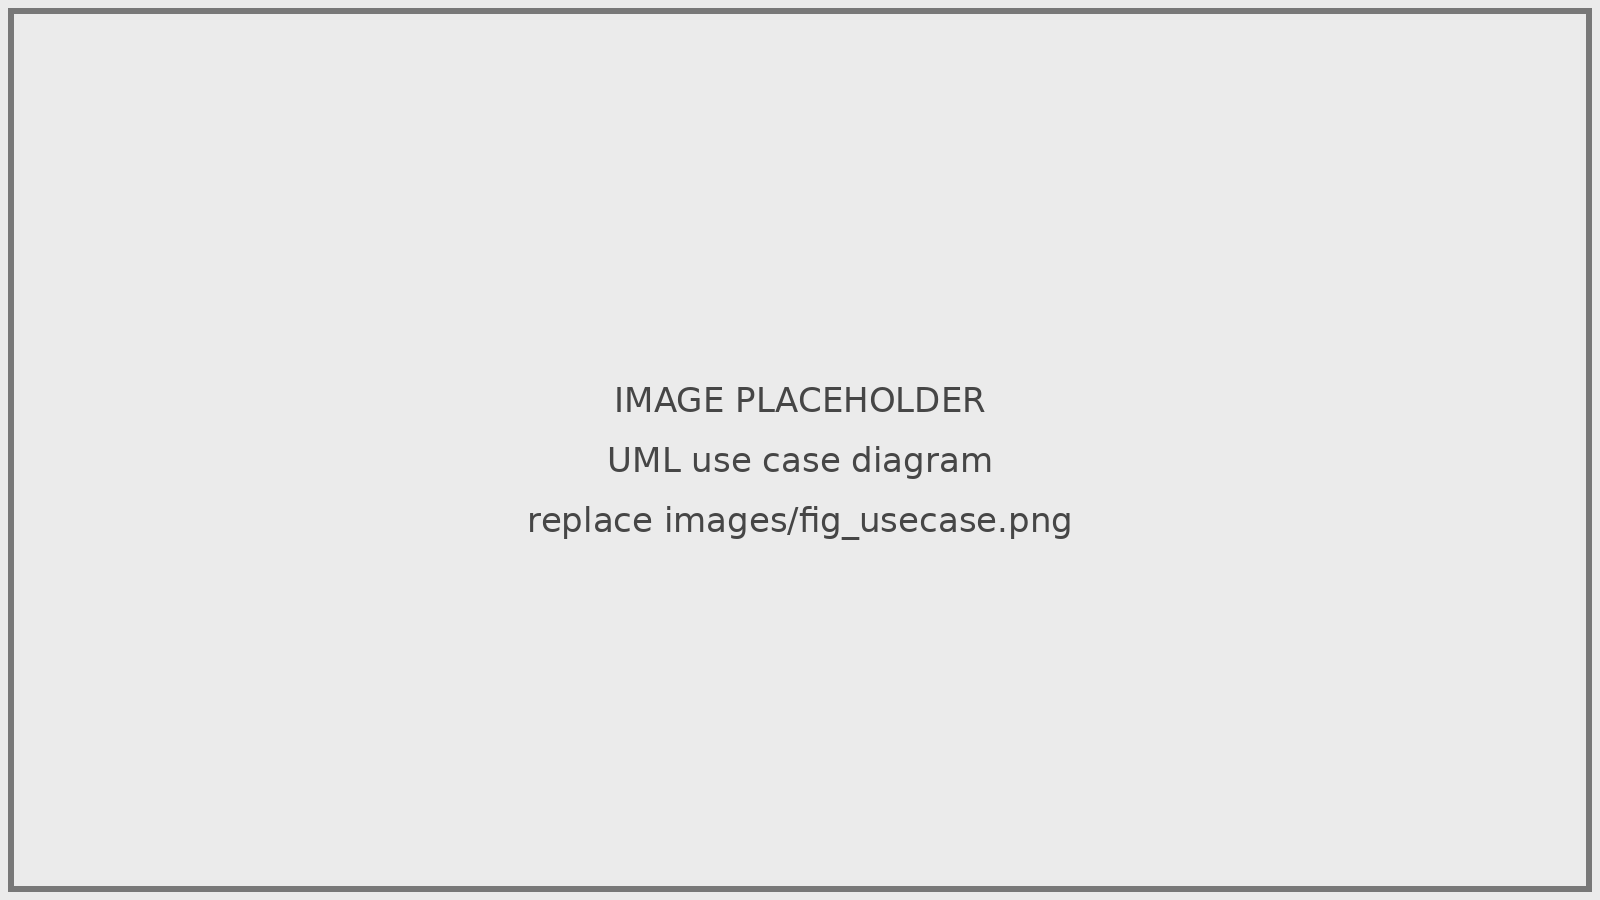
\includegraphics[width=0.8\textwidth]{fig_usecase.png}
	\caption{UML use case diagram}
	\label{fig:usecase}
\end{figure}

\subsection{Sequence Diagram}

Fig.~\ref{fig:sequence} follows one build. The browser posts the prompt to the API, which creates a run and starts the LangGraph graph in a worker. Each agent's ledger entries are streamed back to the browser over SSE. The Validator calls the sandbox, and on failure the Classifier and Reflector loop runs, with the Reflector calling the LLM and its tools. When the run succeeds, the Packager stores the zip and registers the preview, and the browser loads the live app through the preview proxy.

\begin{figure}[!ht]
	\centering
		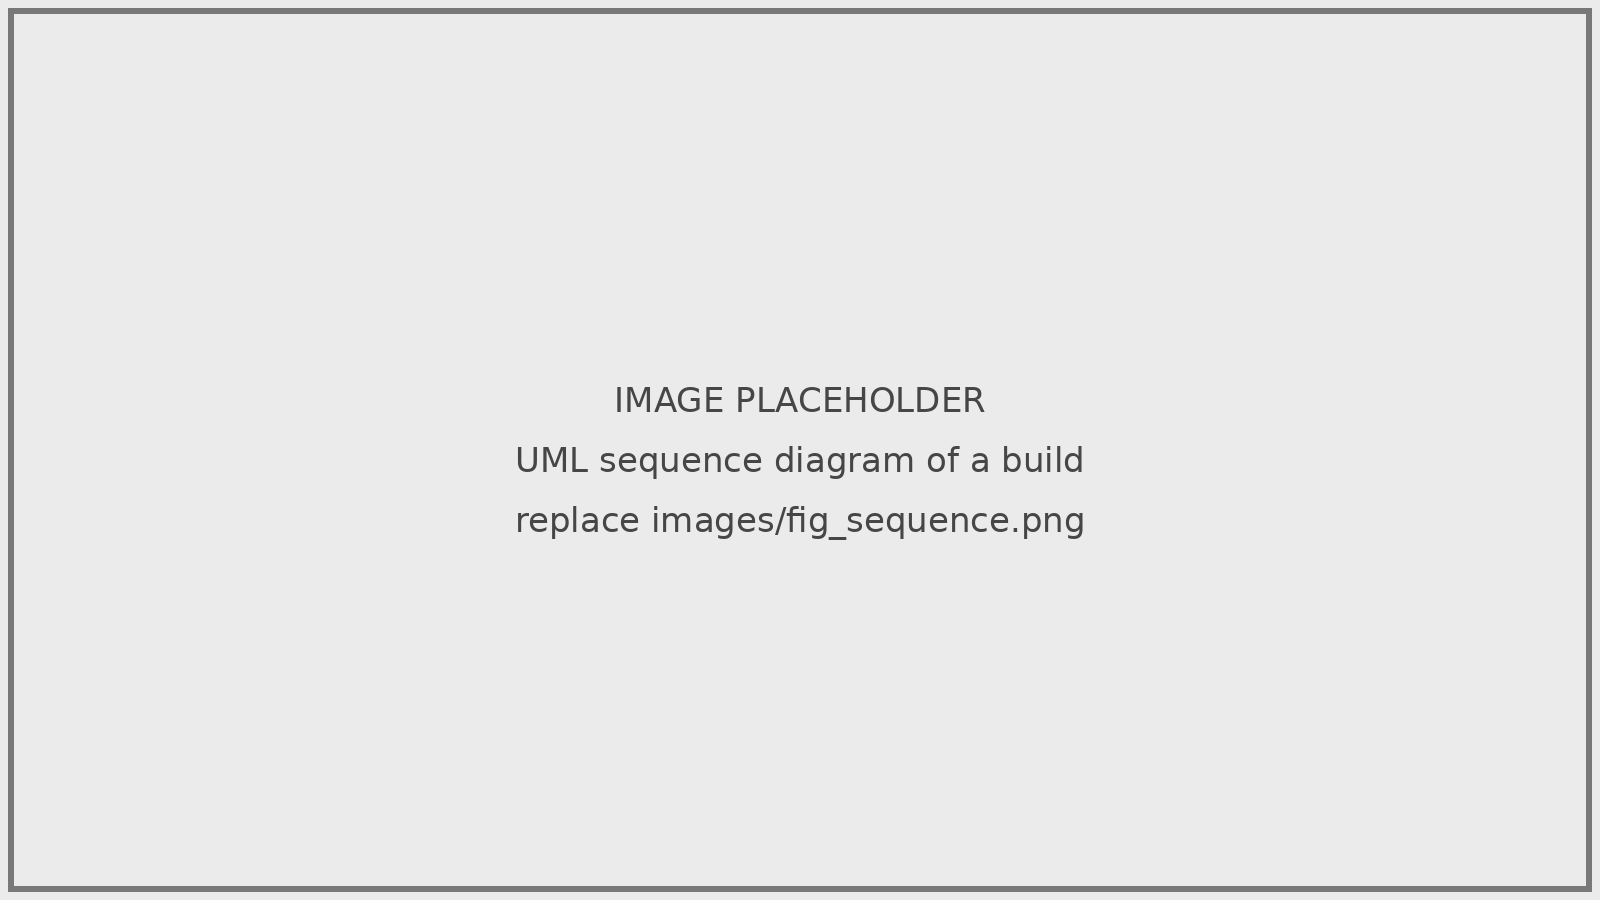
\includegraphics[width=0.85\textwidth]{fig_sequence.png}
	\caption{UML sequence diagram of a build}
	\label{fig:sequence}
\end{figure}

\subsection{Data Flow Diagram}

At Level 0, the user's description goes in, and a verified application, a ledger and a live preview come out, with the LLM provider as an external entity. At Level 1 (Fig.~\ref{fig:dfd}), the data passes through the design (\texttt{ProjectSpec}), the file plan, the generated files, the validation results and the healing history, and is finally stored as an artifact and as a project version.

\begin{figure}[!ht]
	\centering
		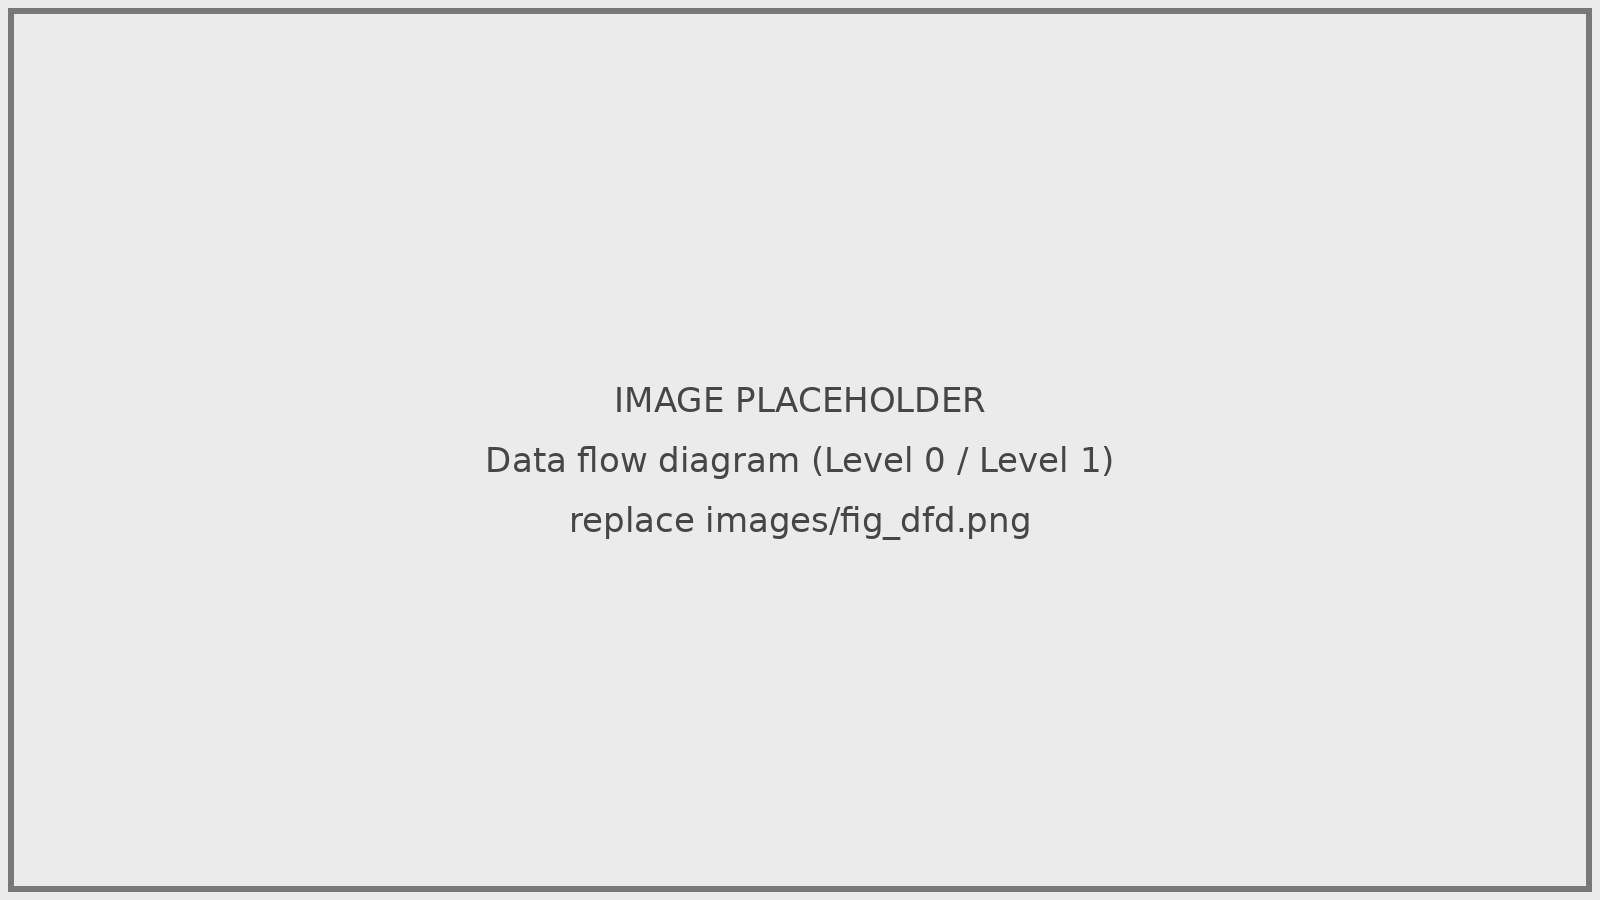
\includegraphics[width=0.85\textwidth]{fig_dfd.png}
	\caption{Data flow diagram}
	\label{fig:dfd}
\end{figure}

\subsection{Entity-Relationship Diagram}

The platform stores \textbf{users}, \textbf{projects} owned by users, \textbf{versions} (runs) belonging to a project, each with its spec, files, status, usage and artifact location, and the \textbf{ledger entries} of each run. LangGraph keeps its own \textbf{checkpoint} tables in the same database, keyed by run. Fig.~\ref{fig:er} shows these relations.

\begin{figure}[!ht]
	\centering
		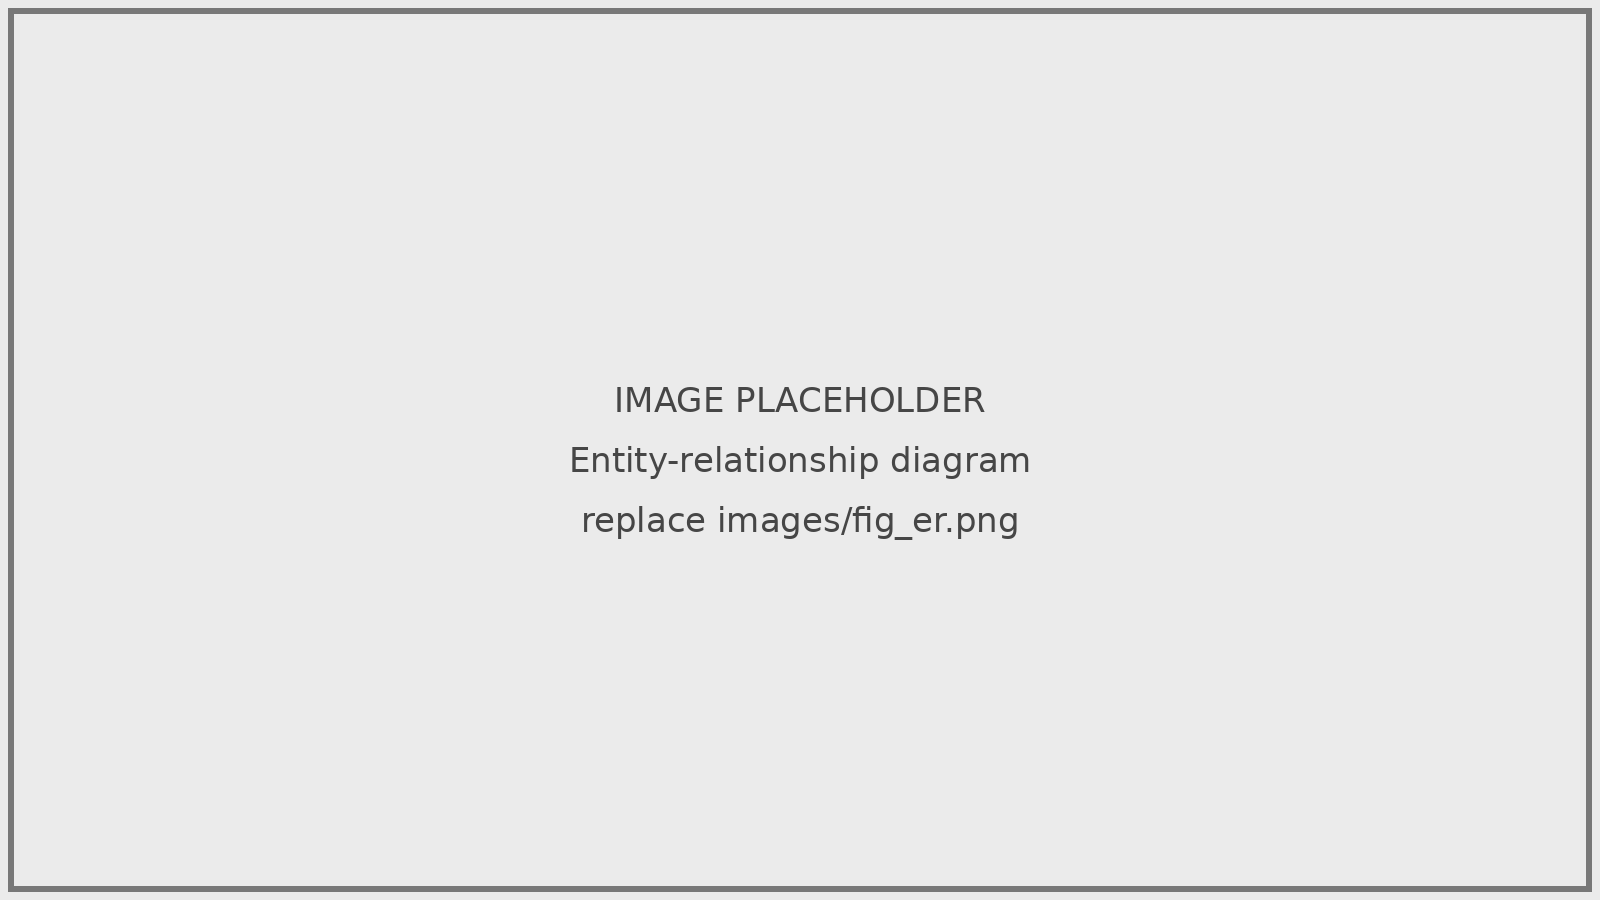
\includegraphics[width=0.75\textwidth]{fig_er.png}
	\caption{Entity-relationship diagram of the platform database}
	\label{fig:er}
\end{figure}

\section{Hardware and Software Specifications}

The language models are reached through hosted APIs, so no GPU is needed for development or deployment. Table~\ref{tab:hw} and Table~\ref{tab:sw} list the requirements.

\begin{table}[!ht]
    \centering
    \renewcommand{\arraystretch}{1.3}
    \caption{Hardware specifications}
    \label{tab:hw}
    \begin{tabular}{|p{4cm}|p{9cm}|}
    \hline
    \textbf{Item} & \textbf{Specification} \\\hline
    Development machine & 4-core CPU, 8\,GB RAM, 10\,GB free disk \\\hline
    Deployment (cloud) & Railway container, 1 vCPU, 1\,GB RAM, persistent volume at \texttt{/data} \\\hline
    GPU & Not required (models are API-hosted) \\\hline
    Network & Internet access to the LLM provider API \\\hline
    \end{tabular}
\end{table}

\begin{table}[!ht]
    \centering
    \renewcommand{\arraystretch}{1.3}
    \caption{Software specifications}
    \label{tab:sw}
    \begin{tabular}{|p{4cm}|p{9cm}|}
    \hline
    \textbf{Item} & \textbf{Specification} \\\hline
    Operating system & Linux (container), also runs on Windows/macOS for development \\\hline
    Languages & Python 3.11, TypeScript \\\hline
    Runtime & Node.js 22 (frontend build only) \\\hline
    Agent framework & LangGraph \\\hline
    Backend frameworks & FastAPI, SQLAlchemy 2.0, Pydantic v2; Flask and Django for generated apps \\\hline
    Frontend & Next.js, React, Tailwind CSS \\\hline
    Database & SQLite (local), PostgreSQL (production) \\\hline
    Testing & pytest, Playwright (browser smoke test) \\\hline
    Deployment & Docker, Docker Compose, Railway; Kubernetes manifests \\\hline
    LLM access & Gemini (default), Groq, OpenRouter or any OpenAI-compatible API \\\hline
    \end{tabular}
\end{table}

% 13. Chapter 4 - System Implementation
\chapter{System Implementation}

This chapter describes how the design was turned into working software. All of the code described here is merged into the main branch of the project repository.

\section{Technology Stack}

Table~\ref{tab:tech} lists the main technologies and why each was chosen. One choice deserves a comment. The platform itself is written in FastAPI with SQLAlchemy and Pydantic, the same stack it generates. This meant that the patterns we wrote into the templates were patterns we were already using and testing every day.

\begin{table}[!ht]
    \centering
    \renewcommand{\arraystretch}{1.3}
    \caption{Technology stack and reasons for selection}
    \label{tab:tech}
    \begin{tabular}{|p{3.2cm}|p{4.2cm}|p{6.2cm}|}
    \hline
    \textbf{Category} & \textbf{Choice} & \textbf{Why it was selected} \\\hline
    Languages & Python 3.11, TypeScript & Python for the AI ecosystem and as the output language; TypeScript for a type-safe UI \\\hline
    Backend framework & FastAPI, SQLAlchemy 2.0, Pydantic v2 & Async, automatic API docs, typed models; the same stack we generate \\\hline
    Agent orchestration & LangGraph & State machine with loops and checkpoints, which suits the heal cycle \\\hline
    LLM access & Gemini, Groq, OpenRouter, OpenAI-compatible & One client with role-based routing, fallback and cost tracking \\\hline
    Frontend & Next.js, React, Tailwind CSS & Static export served by FastAPI; fast and projector-friendly \\\hline
    Database & SQLite / PostgreSQL & Zero-setup locally, robust in production; also holds the checkpoints \\\hline
    Protocols & HTTP/REST, SSE, JWT, MCP & SSE streams agent progress live; JWT secures apps; MCP connects AI tools \\\hline
    Libraries & Jinja2, httpx, uvicorn, pytest & Templates, HTTP calls, app server, tests \\\hline
    Deployment & Docker, Railway, Kubernetes & Low cost, Git-based deploys; Docker for self-hosting \\\hline
    Tools & VS Code, Git/GitHub, ruff, GitHub Actions & Shared tooling, linting, CI \\\hline
    \end{tabular}
\end{table}

\section{Repository Organisation}

The code is organised so that each idea lives in one file:

\begin{singlespace}
\begin{verbatim}
backend/
  agent/          the harness
    graph.py        LangGraph wiring of the 8 agents + CLI
    nodes.py        one function per agent
    state.py        the design (ProjectSpec) and graph state
    healing.py      error classes, fault localisation, stopping rule
    tools.py        the Reflector's tools
    sandbox.py      import -> boot -> tests with OS limits
    bughunt.py      static checks
    testwriter.py   rule tests, calibration, judge
    codegen.py      template rendering, edge-case tests
    stacks.py       FastAPI / Flask / Django specifics
    frontend.py     frontend config and contract check
    llm.py          provider client: tiers, fallback, cost
    templates/      verified templates
  app/            the platform: accounts, projects, runs, SSE,
                  previews, MCP server, queue and worker, deploy
  plugins/        example plugins
  evals/          benchmark prompts and runner
  tests/          automated tests
frontend/         Next.js user interface
deploy/k8s/       Kubernetes manifests
\end{verbatim}
\end{singlespace}

\section{Agent Orchestration}

The graph is built in \texttt{agent/graph.py}. Each of the eight agents is added as a node, and the edges encode the flow described in Chapter~3. The only decision point in the loop is \texttt{route\_after\_validate}, which sends the state to the Packager, the Error Classifier or the Circuit Breaker:

\begin{singlespace}
\begin{verbatim}
g.add_edge("parse_spec", "plan")
g.add_conditional_edges("plan",
    lambda s: "parse_spec" if s.get("design_feedback")
              else "generate")
g.add_edge("generate", "validate")
g.add_conditional_edges("validate",
    nodes.route_after_validate,
    ["package", "classify", "failure_report"])
g.add_edge("classify", "reflect")
g.add_edge("reflect", "validate")
\end{verbatim}
\end{singlespace}

A checkpointer (SQLite locally, PostgreSQL in production) saves the state after every node. This is what makes ``resume after redeploy'' and ``keep fixing'' possible: a run can be continued from its last checkpoint, or restarted at the Validator with the previous version's code.

\section{Self-Healing Implementation}

The healing rules are pure functions over the validation log, so they cost no tokens and can be unit-tested directly. The error classifier, for example, is simply an ordered list of patterns:

\begin{singlespace}
\begin{verbatim}
_RULES = [
  ("sandbox",  SANDBOX_LIMIT),
  ("frontend", re.compile(r"FrontendContractError")),
  ("static",   re.compile(r"StaticCheckError")),
  ("timeout",  re.compile(r"TimeoutError")),
  ("syntax",   re.compile(r"\b(SyntaxError|IndentationError)\b")),
  ...
  ("contract", re.compile(r"AssertionError|\bFAILED\b")),
]
\end{verbatim}
\end{singlespace}

The stopping rule reads the healing history and returns both a decision and a human-readable reason. The reason is shown to the user and written to the ledger, so there is never a silent stop:

\begin{singlespace}
\begin{verbatim}
def should_continue(history, tokens_used, token_budget,
                    llm_available, safety_limit, budget_problem=None):
    attempts = len(history) - 1
    if attempts >= safety_limit:
        return False, "safety limit reached"
    if attempts > 0 and budget_problem:
        return False, budget_problem
    ...   # repeated fingerprint, ladder used up -> stop
\end{verbatim}
\end{singlespace}

\section{Generated Applications}

Every generated project has the same layout in all three frameworks, so the same tests, error classifier and healing loop work unchanged. A generated project includes:

\begin{itemize}
    \item \textbf{Backend:} models, schemas, services, routers, authentication (scrypt password hashing, JWT access tokens, optional rotating refresh tokens with reuse detection), RFC 7807 error responses \cite{rfc7807}, request IDs with JSON logs, \texttt{/health} and \texttt{/ready} endpoints, security headers and a Prometheus \texttt{/metrics} endpoint.
    \item \textbf{Optional production features}, each as verified template code with its own tests: account lockout after failed logins, an immutable audit log, token-bucket rate limiting (shared through Redis when configured), row locks for actions that move money or stock, and live updates over SSE.
    \item \textbf{Frontend:} a complete React and Tailwind app with no build step: login, a dashboard, a page per entity, forms built from the field rules, state and action buttons, and live updates.
    \item \textbf{Database:} Alembic or Django migrations, generated and applied once during validation.
    \item \textbf{Tests:} contract, edge-case and rule tests.
    \item \textbf{Delivery:} a Dockerfile, docker-compose, a Makefile, a CI workflow, a README and the ledger.
\end{itemize}

\section{The Platform}

\textbf{Accounts, projects and versions.} Users sign up and own projects. A project works like a chat: the first message builds version 1, and a follow-up such as ``add reviews with a 1--5 rating'' makes the Architect edit the design. Only the changed business logic is regenerated, the whole app is re-validated as version 2, and any earlier version can be restored. Storage uses SQLAlchemy Core over SQLite or PostgreSQL.

\textbf{Live progress and preview.} Agent progress is streamed over SSE. A draft preview built from the verified screens opens within about a minute, while the business logic is still being written. The final app runs in the sandbox behind a private \texttt{/preview/<key>/} link and is shown in desktop and phone views.

\textbf{Guided prompts and project rules.} The home page offers six starter apps and a step-by-step prompt builder. Per-project rules entered by the user are passed to every agent.

\textbf{Plugins and MCP.} A plugin is a single Python file that can add files, static checks, prompt rules or tools (\texttt{agent/plugins.py}). Nine example plugins are included, among them deploy configurations, seed data, OpenAPI and Postman export, and a secrets scan. The Architect chooses which plugins a build needs. VibeStack is also an MCP server at \texttt{/mcp/}, so assistants in Claude Desktop, Cursor or VS Code can build and edit projects, and it is an MCP client, so the Reflector can use tools from other MCP servers bundled in the container.

\textbf{Scaling and operations.} With \texttt{RUN\_QUEUE=redis}, web servers queue builds in Redis and any number of workers build them. A worker that dies hands its runs to the others, which continue from the last checkpoint. The platform has readiness checks, back-pressure, login rate limits, JSON logs, a Prometheus endpoint and optional Sentry. A passing version can be deployed to a connected Kubernetes cluster in one click. It gets its own namespace, PostgreSQL, a migration job, two replicas and an Ingress, and the public URL is smoke-tested before the app is marked live.

\section{User Interface}

The interface follows a prompt-first design. The home page (Fig.~\ref{fig:uihome}) takes the description and the framework choice. The design review screen (Fig.~\ref{fig:design}) shows the entities, permissions and actions for approval. The workspace (Fig.~\ref{fig:workspace}) has the chat on the left and, on the right, the live pipeline of agents, the generated files, the tests, the ledger and the running app. The quality view (Fig.~\ref{fig:ledger}) lists the bugs the agents found, the tool calls the Reflector made and the fix diffs.

\begin{figure}[!ht]
	\centering
		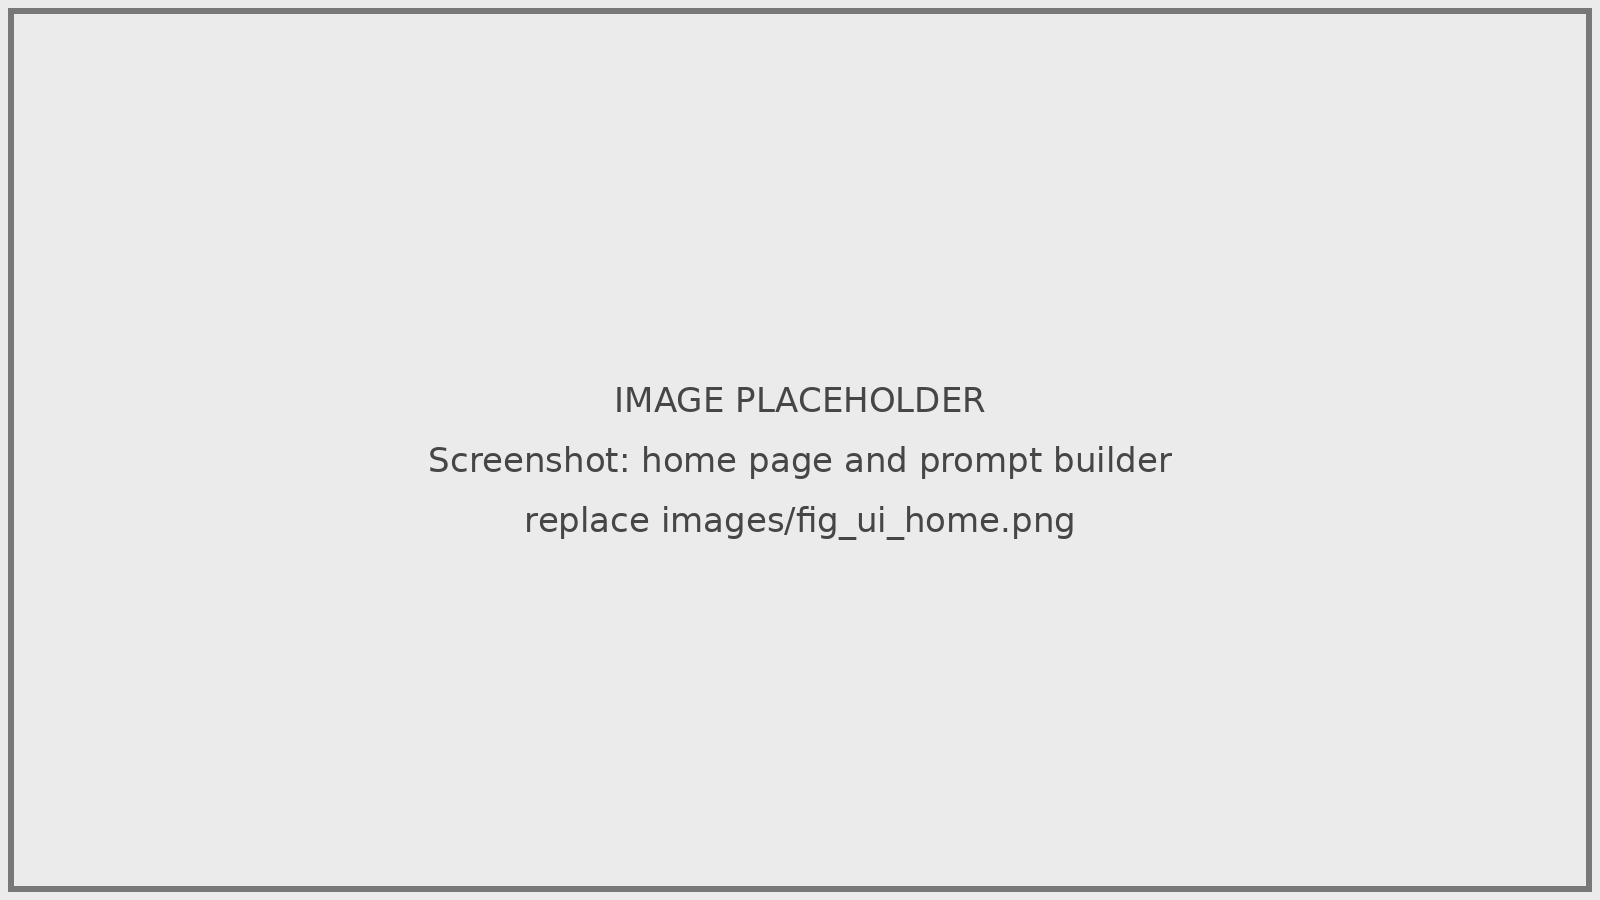
\includegraphics[width=0.85\textwidth]{fig_ui_home.png}
	\caption{Home page with the guided prompt builder}
	\label{fig:uihome}
\end{figure}

\begin{figure}[!ht]
	\centering
		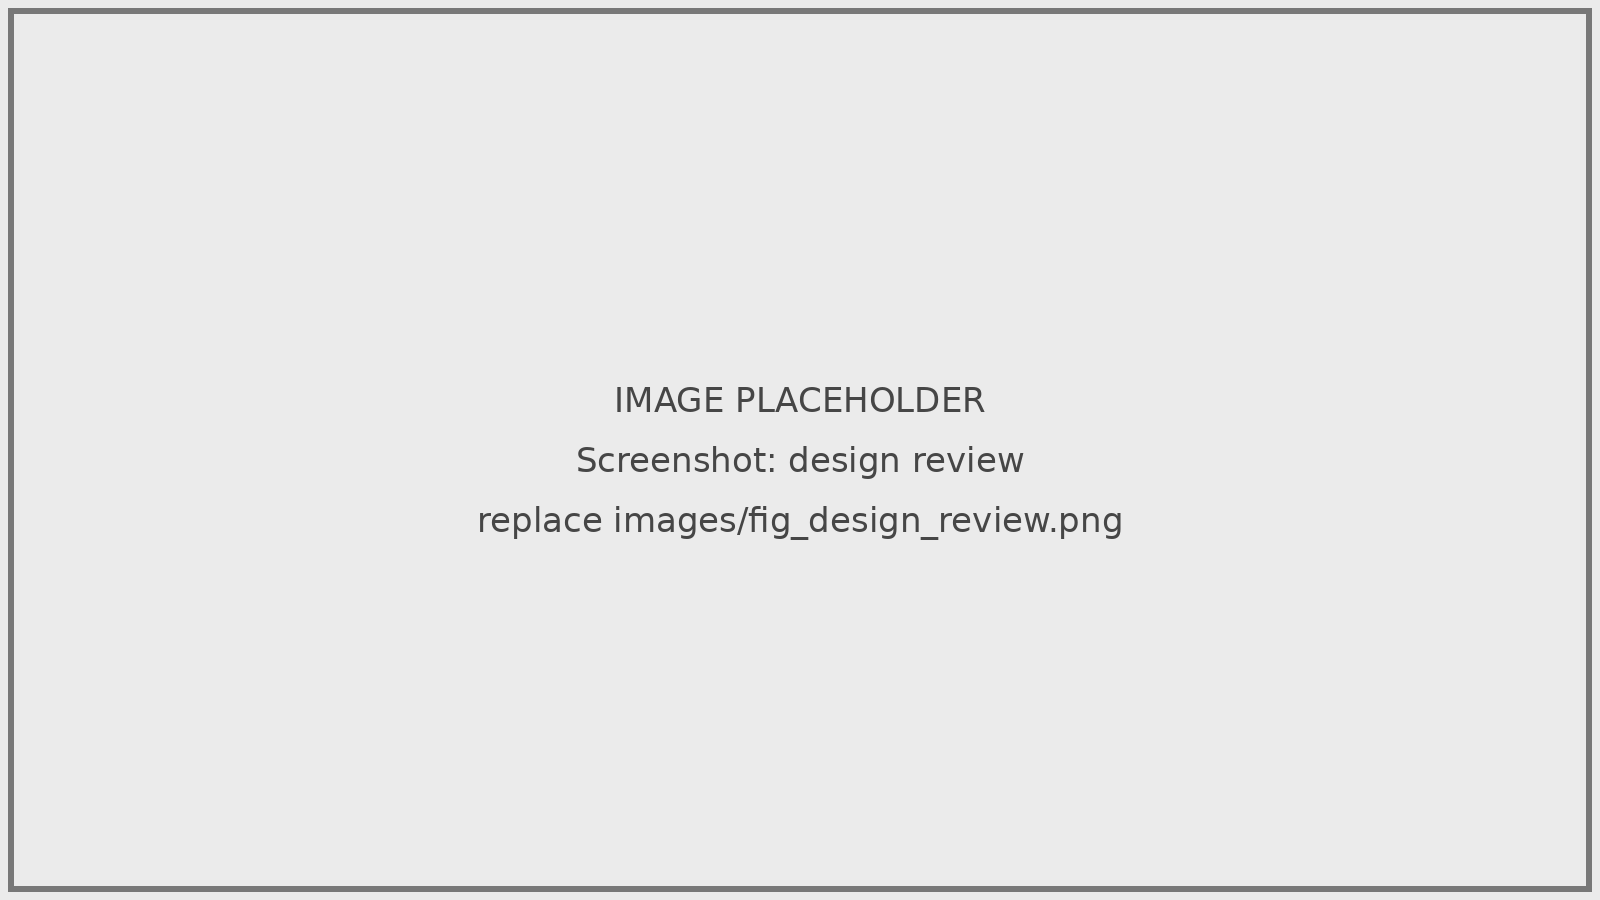
\includegraphics[width=0.85\textwidth]{fig_design_review.png}
	\caption{Design review before code generation}
	\label{fig:design}
\end{figure}

\begin{figure}[!ht]
	\centering
		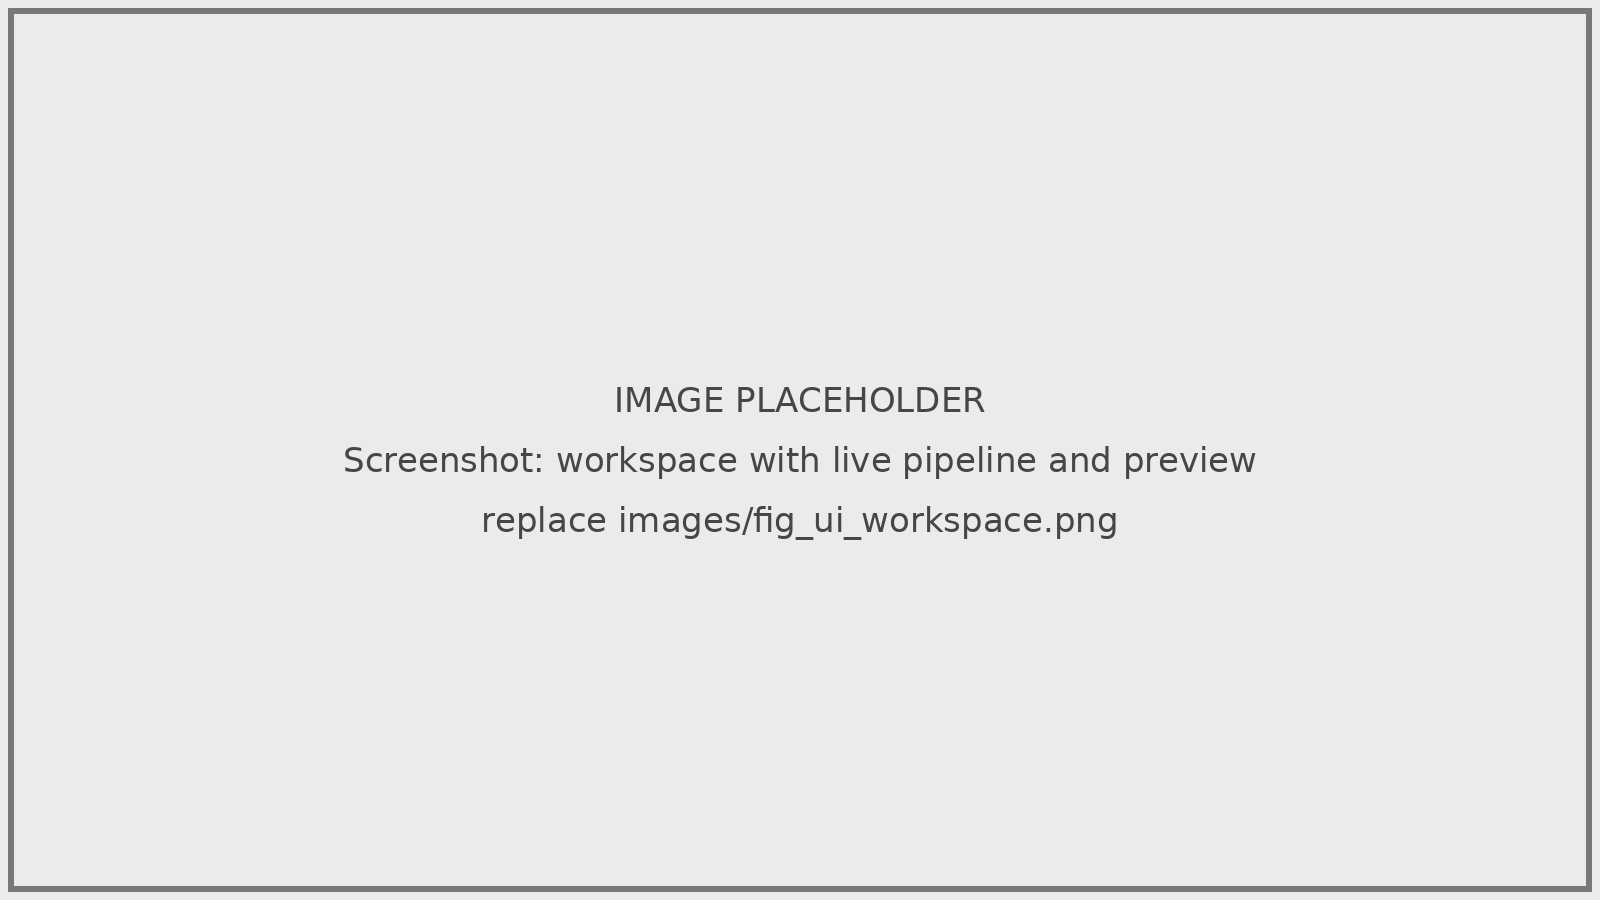
\includegraphics[width=0.85\textwidth]{fig_ui_workspace.png}
	\caption{Project workspace with the live agent pipeline and app preview}
	\label{fig:workspace}
\end{figure}

\begin{figure}[!ht]
	\centering
		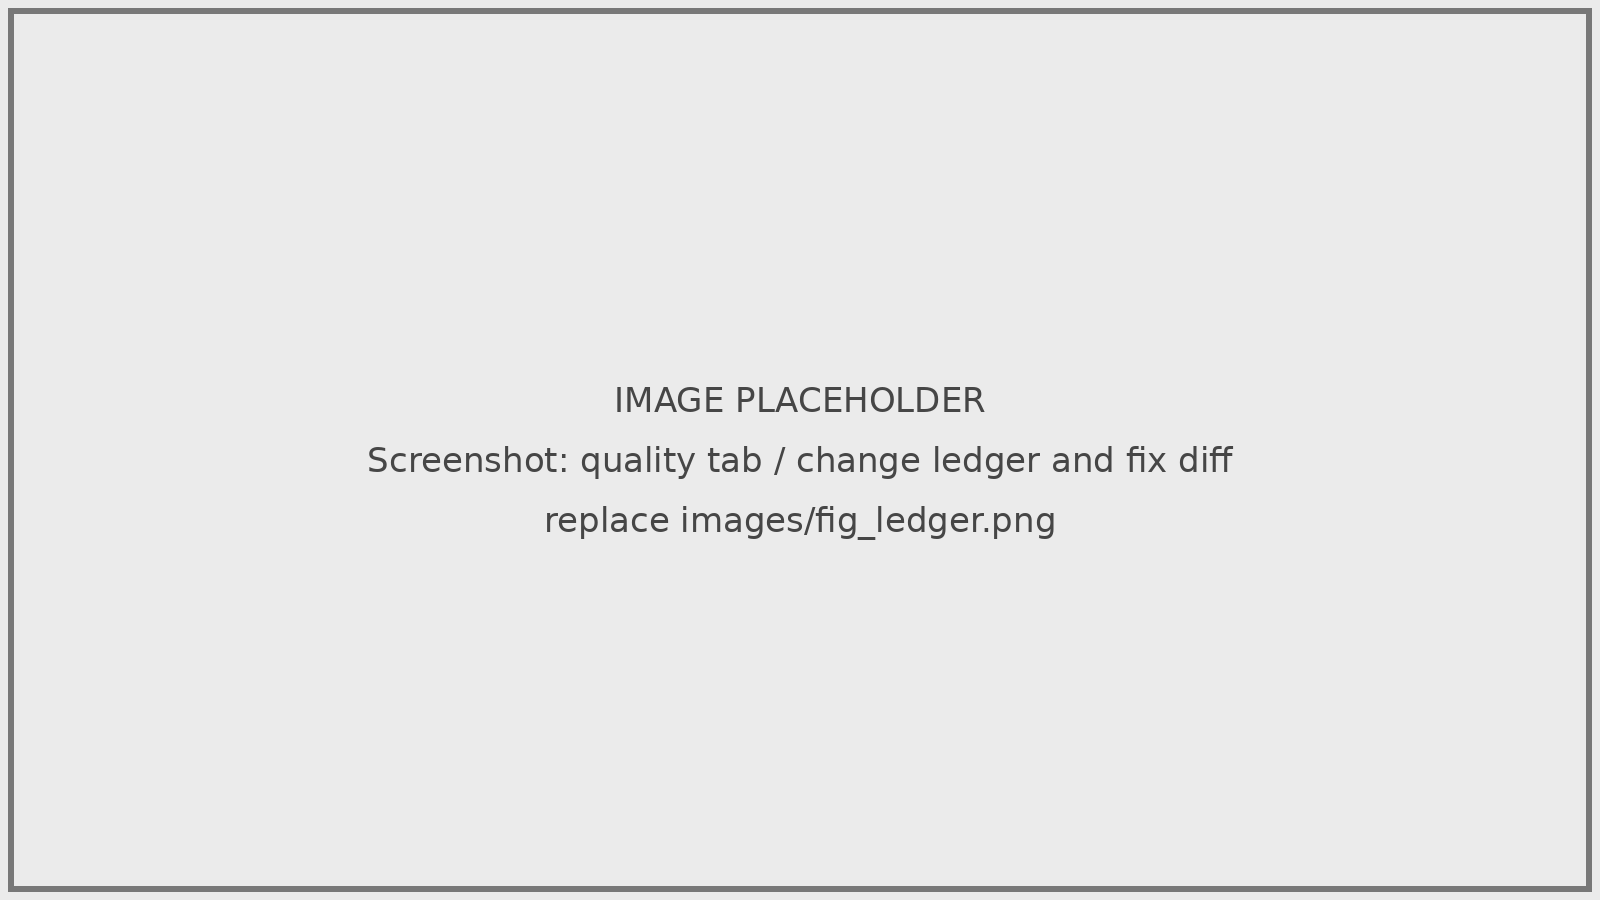
\includegraphics[width=0.85\textwidth]{fig_ledger.png}
	\caption{Quality view showing the change ledger and a fix diff}
	\label{fig:ledger}
\end{figure}

\section{Testing Approach}

Testing an LLM system is tricky because the model's output changes from call to call. We solved this with a deterministic fake model (\texttt{agent/fake\_llm.py}) that returns fixed, realistic answers. With it, the whole graph, including the sandbox, all three frameworks and the healing loop, runs in CI without any API key or token cost. Real-model behaviour is checked separately with \texttt{scripts/check\_llm.py} and with the benchmark runner. GitHub Actions runs the platform tests on a real PostgreSQL database and runs a browser smoke test of the interface.

% 15. Chapter 5 - Preliminary Results
\chapter{Preliminary Results}

This chapter reports what has been measured so far. We have been careful to separate results from the automated test suite, which are fully reproducible, from the single real-model measurements taken for Review 1, and from the benchmark evaluation that is still in progress.

\section{Automated Test Suite}

The repository contains about 120 automated tests across 17 test files (Table~\ref{tab:tests}). They run with the deterministic fake model and a real sandbox, so every run executes generated FastAPI, Flask and Django applications for real. All of them pass on the main branch. At Review 1 the suite had 36 tests. It has grown as features were added, and each new feature came with its own tests.

\begin{table}[!ht]
    \centering
    \renewcommand{\arraystretch}{1.2}
    \caption{Automated tests by area (main branch)}
    \label{tab:tests}
    \begin{tabular}{|p{4.6cm}|p{7.2cm}|c|}
    \hline
    \textbf{Test file} & \textbf{What it checks} & \textbf{Tests} \\\hline
    \texttt{test\_healing.py} & Error classes, localisation, progress and stopping rules & 23 \\\hline
    \texttt{test\_graph.py} & End-to-end graph runs, healing, follow-ups & 13 \\\hline
    \texttt{test\_tools.py} & Reflector tools and tool limits & 12 \\\hline
    \texttt{test\_api.py} & Platform HTTP API & 9 \\\hline
    \texttt{test\_plugins.py} & Plugin loading and hooks & 9 \\\hline
    \texttt{test\_codegen.py} & Template rendering, edge-case tests & 8 \\\hline
    \texttt{test\_spec.py} & \texttt{ProjectSpec} validation & 7 \\\hline
    \texttt{test\_ops.py} & Operations: limits, health, metrics & 7 \\\hline
    \texttt{test\_testwriter.py} & Rule tests, calibration, judge & 7 \\\hline
    \texttt{test\_deploy.py} & Kubernetes deployment & 6 \\\hline
    \texttt{test\_queue.py} & Redis queue and workers & 6 \\\hline
    \texttt{test\_bughunt.py} & Static checks & 5 \\\hline
    \texttt{test\_robustness.py} & Stops, deadlines, idempotent starts & 5 \\\hline
    \texttt{test\_frontend.py} & Frontend contract check & 3 \\\hline
    \texttt{test\_projects.py} & Projects and versions & 3 \\\hline
    \texttt{test\_evals.py}, \texttt{test\_storage.py},\newline \texttt{test\_mcp.py} & Eval runner, storage, MCP server & 5 \\\hline
    \textbf{Total} & & \textbf{121} \\\hline
    \end{tabular}
\end{table}

\section{Benchmark Suite}

The benchmark (\texttt{backend/evals/prompts.yaml}) has 15 prompts. Ten are \textbf{standard} applications: todo, blog, library, e-commerce, clinic, event ticketing, fitness tracker, helpdesk, recipes and fleet management. Five are \textbf{hard} prompts with business rules, permissions and custom actions: checkout, clinic, library, project management and ticketing. Each prompt also has a reference spec, so the harness can be tested offline without a model.

\section{Interim Measurements (Review 1)}

The following numbers were measured for the Review 1 interim evaluation on 8 October 2026, on the version of the system that existed at that time.

\begin{table}[!ht]
    \centering
    \renewcommand{\arraystretch}{1.3}
    \caption{Interim measurements reported at Review 1}
    \label{tab:interim}
    \begin{tabular}{|p{7cm}|p{6cm}|}
    \hline
    \textbf{Measurement} & \textbf{Value} \\\hline
    End-to-end real run on Railway (blog app with JWT auth) & about 51 seconds \\\hline
    API cost of that run & US\$0.009 (about 9.6k tokens) \\\hline
    Gates passed in that run & 3 of 3 (import, boot, API tests) \\\hline
    Benchmark projects healed (planted-bug harness evaluation) & 10 of 10 \\\hline
    Repair iterations needed per planted bug & 1 \\\hline
    \end{tabular}
\end{table}

The planted-bug evaluation was a deliberate test of the healing loop: a known bug was inserted into each of the ten benchmark projects to check that the loop could find and fix it. Since Review 1, planted bugs have been removed from the system entirely. The agents now have to find real bugs on their own, through the static checks, edge-case tests and rule tests. This is a harder and more honest test, and it is what the Phase II benchmark will measure.

\section{Performance Indicators}

Table~\ref{tab:kpi} compares the targets we set at the start with what the prototype has achieved so far.

\begin{table}[!ht]
    \centering
    \renewcommand{\arraystretch}{1.3}
    \caption{Expected and achieved performance indicators}
    \label{tab:kpi}
    \begin{tabular}{|p{5cm}|p{3.8cm}|p{4.8cm}|}
    \hline
    \textbf{Performance indicator} & \textbf{Expected} & \textbf{Achieved (prototype)} \\\hline
    Architecture produced from a prompt & Valid, schema-checked spec & Yes, on every run \\\hline
    Generated app passes all gates & $\geq$ 80\% of benchmark prompts & 10/10 after healing (Review 1 harness evaluation) \\\hline
    Repair attempts per failure & Bounded, without giving up early & 1 on the planted-bug runs; now progress-driven \\\hline
    API cost per generated app & $<$ US\$0.25 & US\$0.009 with budget models, about US\$0.20 with a strong model \\\hline
    Frameworks supported & FastAPI & FastAPI, Flask and Django \\\hline
    \end{tabular}
\end{table}

\section{Planned Evaluation and Ablation Design}

The evaluation runner (\texttt{backend/evals/run.py}) is complete and runs end to end offline. For each prompt and framework it reports the pass rate, first-try passes, the number of repairs, the bugs found and fixed, \emph{escaped} bugs, tool calls, tokens, cost and time, and it writes the results as Markdown, JSON and CSV. Escaped bugs are counted on a held-out run of the edge-case tests, and of any rule tests a configuration did not use, against the final code.

To measure what each idea contributes, the runner compares the full system with four variants:
\begin{itemize}
    \item \textbf{fixed-3:} healing limited to a fixed three repairs;
    \item \textbf{no-tools:} a one-shot Reflector without tools;
    \item \textbf{no-calibration:} rule tests are not checked against the verified templates;
    \item \textbf{no-rule-tests:} the Architect's rule tests are kept out of validation.
\end{itemize}

Running this benchmark on real models across all three frameworks is the main evaluation task for Phase II. We have deliberately not reported numbers from it here because those runs are not complete.

% 16. Chapter 6 - Project Schedule
\chapter{Project Schedule}

Fig.~\ref{fig:gantt} shows the Gantt chart for the project. Table~\ref{tab:milestones} lists the milestones reached so far, with dates taken from the review schedule and the project's commit history, and Table~\ref{tab:remaining} lists the work that remains.

\begin{figure}[!ht]
	\centering
		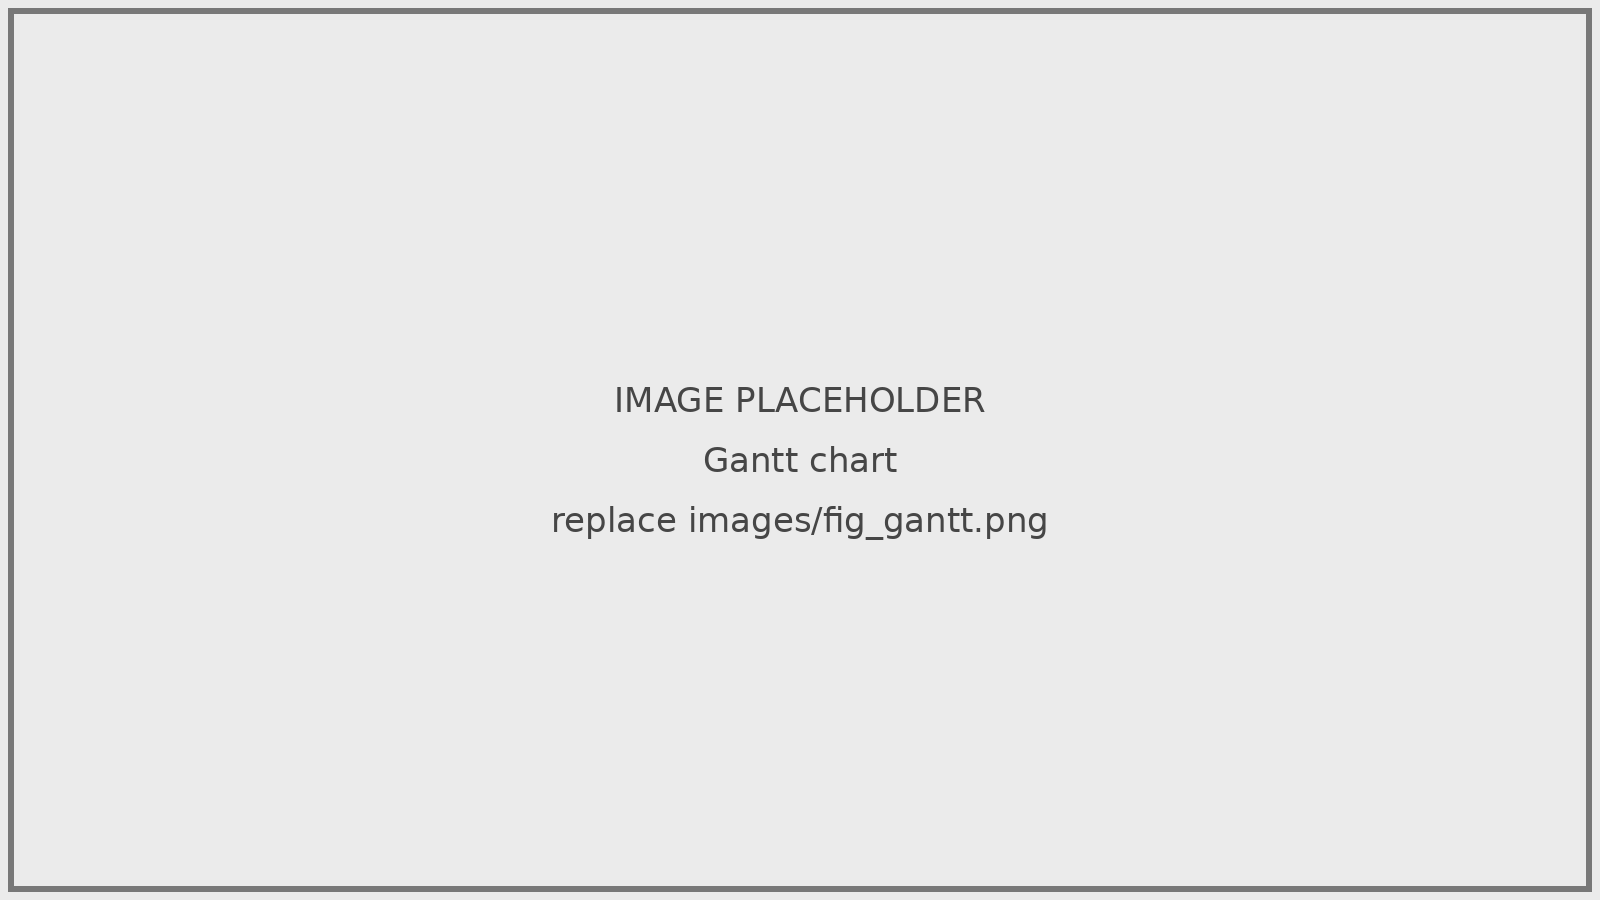
\includegraphics[width=0.95\textwidth]{fig_gantt.png}
	\caption{Gantt chart of the project}
	\label{fig:gantt}
\end{figure}

\begin{table}[!ht]
    \centering
    \renewcommand{\arraystretch}{1.3}
    \caption{Milestones completed}
    \label{tab:milestones}
    \begin{tabular}{|p{3.2cm}|p{10.3cm}|}
    \hline
    \textbf{Date} & \textbf{Milestone} \\\hline
    Aug 2026 & Literature survey and zeroth review \\\hline
    Aug--Sep 2026 & Design: architecture, data flow diagrams, agent roles \\\hline
    5 Oct 2026 & First working harness: LangGraph pipeline with self-healing for FastAPI backends \\\hline
    7 Oct 2026 & Live preview of generated apps; projector-friendly UI with live pipeline and fix diffs \\\hline
    8 Oct 2026 & Review 1 (interim evaluation) \\\hline
    14 Oct 2026 & Planted bugs removed; progress-driven healing; Flask and Django support; accounts, quotas, sandbox limits, CI; MCP server and plugins \\\hline
    16 Oct 2026 & Full-stack apps with React frontend; projects with follow-up edits; tool-using Reflector; ablation evaluation; provider switch \\\hline
    17 Oct 2026 & AI writes only business logic; rule-test calibration; production features as templates; Redis workers; Kubernetes manifests \\\hline
    18 Oct 2026 & Design review before code; agents choose plugins; one-click Kubernetes deploy; multi-file repairs; build deadlines; bundled MCP tool servers \\\hline
    \end{tabular}
\end{table}

\begin{table}[!ht]
    \centering
    \renewcommand{\arraystretch}{1.3}
    \caption{Remaining work and planned timeline}
    \label{tab:remaining}
    \begin{tabular}{|p{2.8cm}|p{7.2cm}|p{3.4cm}|}
    \hline
    \textbf{Activity} & \textbf{Deliverable} & \textbf{Planned period} \\\hline
    Testing & Benchmark report: 15 prompts, 3 frameworks, real models, ablations & Nov 2026 -- Jan 2027 \\\hline
    Optimisation & Lower token cost and latency (prompt caching) & Nov -- Dec 2026 \\\hline
    Security & Trivy / Checkov scan gate added to the sandbox & Dec 2026 \\\hline
    Integration & Long-term memory of past fixes (ChromaDB) & Dec 2026 -- Jan 2027 \\\hline
    Review 2 & Second review & Jan 2027 \\\hline
    Publication & Conference paper on the self-healing harness & Jan -- Mar 2027 \\\hline
    Copyright & Software copyright registration for VibeStack & Feb -- Mar 2027 \\\hline
    Documentation & Final report, user guide, API documentation & Oct 2026 -- Mar 2027 \\\hline
    Final & Final project evaluation and viva & Mar -- Apr 2027 \\\hline
    \end{tabular}
\end{table}

% 16. Chapter 7 - Conclusion
\chapter{Conclusion}

In Phase I we set out to build a system that does not just generate backend code but checks and repairs it before handing it over. That system now exists and is merged into the main branch. Eight agents, connected as a LangGraph state machine, take a plain-English description through design, generation, sandboxed validation and repair, and deliver a full-stack application with a FastAPI, Flask or Django backend and a React frontend, together with its tests, migrations, Docker setup and a ledger of every change.

Three ideas have shaped the system most. First, letting the model write only the business logic, while verified templates provide everything else, made builds faster and removed whole classes of errors. Second, deriving edge-case tests from the design without any AI gave us an independent check that the model cannot game, and calibrating the model's own tests stopped wrong tests from steering the repairs. Third, replacing the fixed three-attempt limit with a progress-based stopping rule means that healing continues while it is helping and stops, with a clear reason, when it is not.

\section{Limitations}

\begin{itemize}
    \item The system targets CRUD-style applications with business rules. Arbitrary algorithms and non-web software are outside its scope.
    \item The full benchmark on real models has not been completed yet, so the success rates and costs reported here come from the test suite and from the Review 1 measurements.
    \item Results depend on the language model provider, and model behaviour can change between versions.
    \item The edge-case tests serve both as part of validation and as the held-out oracle in the evaluation. The evaluation design accounts for this by reporting held-out numbers only for configurations that did not use them.
\end{itemize}

\section{Future Work}

In Phase II we will run the full benchmark of fifteen prompts across three frameworks on real models, with the ablation studies, and report the pass rate, escaped bugs, cost and time. We also plan to add a security scanning gate (Trivy and Checkov) to the sandbox, reduce cost and latency through prompt caching, give the Reflector a memory of past fixes, write a conference paper on progress-driven self-healing, and register the software for copyright.

\singlespacing
% 17. Bibliography
\bibliographystyle{IEEEtran}
\bibliography{references.bib}

% APPENDIX
\appendix
\chapter{Turnitin Plagiarism Report}
[Insert Plagiarism Report Here]

\chapter{Base Paper (most relevant one)}
[Insert Base Paper Here]

\end{document}
